% =====================================================================
%  MSc Dissertation — Heriot-Watt University thesis format
%  (following the HWU submission guidelines as implemented by the
%   Heriot_Watt_Thesis_Template: A4, 40mm left / 20mm other margins,
%   12pt Times-like font, 1.5 line spacing, Roman preliminaries,
%   Arabic main text, 14pt bold chapters, declaration bound in.)
%
%  Compile: pdflatex main && bibtex main && pdflatex main && pdflatex main
% =====================================================================
\documentclass[12pt,a4paper]{report}

% ------------------------- fonts & encoding -------------------------
\usepackage[utf8]{inputenc}
\usepackage[T1]{fontenc}
\usepackage{mathptmx}           % Times New Roman look (per HWU template)
\usepackage[protrusion=true,expansion=false]{microtype}
\usepackage{setspace}
\setstretch{1.5}                % 1.5 line spacing (HWU requirement)

% ------------------------- geometry (HWU: 40mm left, 20mm rest) -----
\usepackage[a4paper,left=40mm,right=20mm,top=20mm,bottom=20mm,
            headheight=20pt,headsep=25pt,footskip=30pt]{geometry}

% ------------------------- page styles -------------------------------
\usepackage{fancyhdr}
% preliminary pages: empty header, Roman page number in footer
\fancypagestyle{preliminary}{%
  \fancyhf{}%
  \renewcommand{\headrulewidth}{0pt}%
  \fancyfoot[C]{\thepage}%
}
% main text: chapter title in header (10pt italics, no bold), Arabic page
% number centred in footer
\fancypagestyle{chapter}{%
  \fancyhf{}%
  \fancyhead[L]{\normalfont\itshape\fontsize{10pt}{12pt}\selectfont\nouppercase{\leftmark}}%
  \fancyhead[R]{}%
  \fancyfoot[C]{\thepage}%
  \renewcommand{\headrulewidth}{0.4pt}%
  \renewcommand{\footrulewidth}{0pt}%
}
\pagestyle{preliminary}

% ------------------------- headings (HWU sizes) ----------------------
\usepackage{titlesec}
% Chapter: 14pt, bold, capitalised initial
\titleformat{\chapter}[display]
  {\normalfont\bfseries\fontsize{14pt}{16.8pt}\selectfont}
  {\chaptertitlename\ \thechapter}{14pt}{}
\titlespacing{\chapter}{0pt}{10pt}{25pt}
% Section: 12pt, bold
\titleformat{\section}[hang]
  {\normalfont\bfseries\fontsize{12pt}{14.4pt}\selectfont}
  {\thesection}{5pt}{}
\titlespacing{\section}{0pt}{25pt}{15pt}
% Subsection: 12pt, bold + italic
\titleformat{\subsection}[hang]
  {\normalfont\bfseries\itshape\fontsize{12pt}{14.4pt}\selectfont}
  {\thesubsection}{5pt}{}
\titlespacing{\subsection}{0pt}{20pt}{10pt}
% Subsubsection: unnumbered, not in ToC (HWU guideline)
\setcounter{tocdepth}{2}
\setcounter{secnumdepth}{2}

% ------------------------- tables & figures -------------------------
\usepackage{graphicx}
\usepackage{booktabs}
\usepackage{longtable}
\usepackage{array}
\usepackage{multirow}
\usepackage{adjustbox}
\usepackage{subcaption}
\usepackage[table]{xcolor}
\usepackage{float}
\usepackage{placeins}
\graphicspath{{figures/}}
\setlength{\textfloatsep}{14pt plus 2pt minus 4pt}
\setlength{\floatsep}{12pt plus 2pt minus 4pt}

% ------------------------- math & lists -----------------------------
\usepackage{amsmath}            % amssymb deliberately omitted: newtxmath already provides its symbols
\usepackage{enumitem}
\setlist{itemsep=2pt,topsep=4pt,parsep=0pt}
\usepackage{caption}
\captionsetup{font=small,labelfont=bf,skip=6pt}

% ------------------------- code listings ----------------------------
\usepackage{listings}
\lstset{
  basicstyle=\ttfamily\small,
  frame=single,
  rulecolor=\color{gray!60},
  backgroundcolor=\color{gray!8},
  breaklines=true,
  columns=fullflexible,
  captionpos=b,
  aboveskip=8pt,
  belowskip=8pt,
}
\usepackage{xcolor}
\definecolor{navy}{RGB}{18,32,49}
\definecolor{blueA}{RGB}{37,99,235}
\definecolor{orangeB}{RGB}{244,122,36}
\definecolor{cyanD}{RGB}{18,184,212}

% ------------------------- references -------------------------------
\usepackage[square,sort&compress,numbers]{natbib}
\renewcommand{\bibname}{References}
\usepackage{url}
\urlstyle{same}
\usepackage[hidelinks]{hyperref}
\hypersetup{
  colorlinks=true,
  linkcolor=navy,
  citecolor=blueA,
  urlcolor=blueA,
  pdftitle={Sonar-Based 3D Reconstruction of Small Underwater Objects: Two Routes for the SUOP Dataset},
  pdfauthor={},
}

% ------------------------- thesis information ------------------------
\newcommand{\thesistitle}{Sonar-Based 3D Reconstruction of Small Underwater
Objects: Two Routes for the \suop{} Dataset}
\newcommand{\authorName}{[Your Full Name]}
\newcommand{\degreeQualification}{Master of Science}
\newcommand{\school}{School of Engineering and Physical Sciences}
\newcommand{\university}{Heriot-Watt University}
\newcommand{\monthDate}{August}
\newcommand{\yearDate}{2026}

% ------------------------- list names --------------------------------
\renewcommand{\contentsname}{Table of Contents}

% ------------------------- custom commands --------------------------
\newcommand{\routeA}{\textbf{Route~A}}
\newcommand{\routeB}{\textbf{Route~B}}
\newcommand{\suop}{\textsc{Suop}}
\newcommand{\pcn}{PCN}
\newcommand{\chd}{Chamfer}
\newcommand{\figref}[1]{Figure~\ref{#1}}
\newcommand{\tabref}[1]{Table~\ref{#1}}
\newcommand{\secref}[1]{Section~\ref{#1}}
\newcommand{\eqrefn}[1]{Equation~\eqref{#1}}
\newcommand{\mm}{\,\text{mm}}
\newcommand{\m}{\,\text{m}}

% =====================================================================
\begin{document}

% ------------------------- preliminaries -----------------------------
% HWU: all preliminaries use Roman numerals; the title page itself is
% unnumbered (empty style). The titlepage environment resets the page
% counter to 1, so the abstract becomes page ii, etc.
\pagestyle{empty}
\pagenumbering{Roman}
% =====================================================================
% Front matter (Heriot-Watt University format):
% Title page -> Abstract (<=200 words, single page) -> Dedication
% -> Acknowledgements -> Declaration (official form bound in)
% =====================================================================

% ------------------------- title page --------------------------------
\begin{titlepage}
\begin{center}
\vspace*{15pt}\par
\setstretch{1}
{\Large\bfseries\MakeUppercase{Sonar-Based 3D Reconstruction of Small
Underwater Objects: Two Routes for the \suop{} Dataset}}\\
\vspace{40pt}\par

\includegraphics[width=140pt]{hwulogo.png}\\
\vspace{40pt}\par
{\itshape\fontsize{15.5pt}{19pt}\selectfont by\\}\vspace{15pt}\par
{\Large\authorName}\vspace{55pt}\par
{\large Submitted for the degree of \\ \vspace{8pt} \Large\slshape\degreeQualification\\}
\vspace{35pt}\par
{\scshape\setstretch{1.5}\school\\ \university\\}
\vspace{50pt}\par
{\large\monthDate\ \yearDate}
\vfill
\begin{flushleft}
\setstretch{1.4}\small
The copyright in this thesis is owned by the author. Any quotation from the
thesis or use of any of the information contained in it must acknowledge this
thesis as the source of the quotation or information.
\end{flushleft}
\end{center}
\end{titlepage}

% ------------------------- abstract ----------------------------------
\chapter*{Abstract}
\addcontentsline{toc}{chapter}{Abstract}

Acoustic sonar point clouds of small underwater objects are partial, noisy and
unevenly sampled, and the \suop{} (Small Underwater Objects 3D Point Cloud)
dataset adds the further difficulty that the pose of the object was not logged
during acquisition. This dissertation investigates how such incomplete returns
can be converted into useful 3D representations, and makes explicit when each
of two complementary routes should be chosen.

\routeA{}, multi-view geometric fusion, estimates the relative poses of
segmented scans with FPFH/RANSAC/ICP, optimises them jointly in a pose graph
with loop closures, fuses the aligned measurements, and surfaces them with
Screened Poisson and ball-pivoting meshing. For all five object categories the
graph connects 24/24 views, and variant pipelines report median
observed-to-surface residuals of $2.9$--$5.0\mm$.

\routeB{}, single-view learned completion, trains a Point Completion Network
with a symmetric Chamfer loss on sonar-realistic partials derived from
procedural models and from \routeA{}'s own meshes. Training converges (final
training Chamfer $1.1\times10^{-3}$--$2.3\times10^{-3}$), and a real chair
partial is completed at the correct scale.

The routes differ in output meaning --- measurement fusion versus
prior-informed inference --- and therefore in evaluation protocol. A
calibrated acquisition with logged poses and an external reference mesh is
proposed as the decisive future experiment.

% ------------------------- dedication --------------------------------
\chapter*{Dedication}
\addcontentsline{toc}{chapter}{Dedication}
To my family, for their patience and support throughout this project.

% ------------------------- acknowledgements -------------------------
\chapter*{Acknowledgements}
\addcontentsline{toc}{chapter}{Acknowledgements}
I would like to thank my supervisor for guidance and feedback throughout this
project, and the IOES-Lab for releasing the \suop{} dataset and its detection
benchmark publicly. I am also grateful to my family and friends for their
patience and support during the writing of this dissertation.

% ------------------------- declaration -------------------------------
\chapter*{Declaration}
\addcontentsline{toc}{chapter}{Declaration}

I hereby declare that the work presented in this dissertation is my own and
that, to the best of my knowledge and belief, it contains no material
previously published or written by another person, except where due
acknowledgement is made in the text. I further declare that this dissertation
has not been submitted, in whole or in part, for any other degree or
professional qualification at this or any other institution.

\vspace{1.5cm}
Signature: \rule{6cm}{0.4pt} \hfill Date: \rule{4cm}{0.4pt}

\vspace{2cm}
{\small\itshape Note: the official Heriot-Watt University Declaration of
Academic Integrity form must be signed and bound into every submitted copy of
the thesis (see the \texttt{Heriot\_Watt\_Thesis\_Template} guidance).}


\pagestyle{preliminary}
\tableofcontents
\clearpage
\listoffigures
\clearpage
\listoftables
\clearpage

% ------------------------- main matter ------------------------------
\pagestyle{chapter}
\pagenumbering{arabic}
\input{chapters/ch01_introduction}
\input{chapters/ch02_literature_review}
\input{chapters/ch03_dataset_preparation}
% =====================================================================
% Chapter 4 — Route A: Multi-View Geometric Fusion
% =====================================================================
\chapter{Route~A: Multi-View Geometric Fusion}
\label{ch:routeA}

This chapter presents the methodology of \routeA, the purely geometric route.
It first justifies \emph{why} Route~A is the appropriate answer in this
project (Section~\ref{sec:why_routeA}), then details the pipeline in its four
stages: pairwise registration (Section~\ref{sec:routea_pairwise}), pose-graph
optimisation (Section~\ref{sec:routea_graph}), fusion (Section~\ref{sec:routea_fusion})
and meshing (Section~\ref{sec:routea_meshing}). Two variants are then described
(Section~\ref{sec:routea_variants}): the view-aware seabed-plane variant and the
sonar-native first-return ray TSDF variant.

\section{Why Route~A?}
\label{sec:why_routeA}

Route~A is the answer to the research question under the following conditions:

\begin{enumerate}
  \item \textbf{Several scans of the same rigid object are available.} The
  \suop{} 3~m acquisition provides 24 curated cases per object, each a
  different placement/orientation of the same physical object. If these scans
  can be aligned into a common frame, each object is observed from many
  effective viewpoints, and the unobserved regions of any single scan are
  covered by the others.
  \item \textbf{The output must be a faithful record of the measurements.}
  Route~A never invents geometry: every point of the output descends from a
  registered sonar return. For safety- and inspection-critical applications
  (e.g.\ estimating whether a propeller is fouled, or whether a net is torn)
  it is preferable to under-cover than to hallucinate, so a measurement-fusion
  route is the defensible choice.
  \item \textbf{No external CAD or learned prior is available or trusted.}
  The \suop{} release contains no CAD models, and the object categories (tyre,
  drum, dummy, net, folding chair) are physically variable, so fitting a rigid
  template would impose assumptions. Route~A requires no prior beyond the
  published object scale used for segmentation.
\end{enumerate}

The \emph{core assumption} of Route~A is that the segmented scans are noisy
partial views of one rigid object, so there exists a set of rigid transforms
that brings them into agreement. The pipeline is therefore a structure-from-scan
problem with unknown poses: registration first, fusion second, meshing third.
Route~A's pipeline is summarised in \figref{fig:routeA_overview}.

\begin{figure}[H]
  \centering
  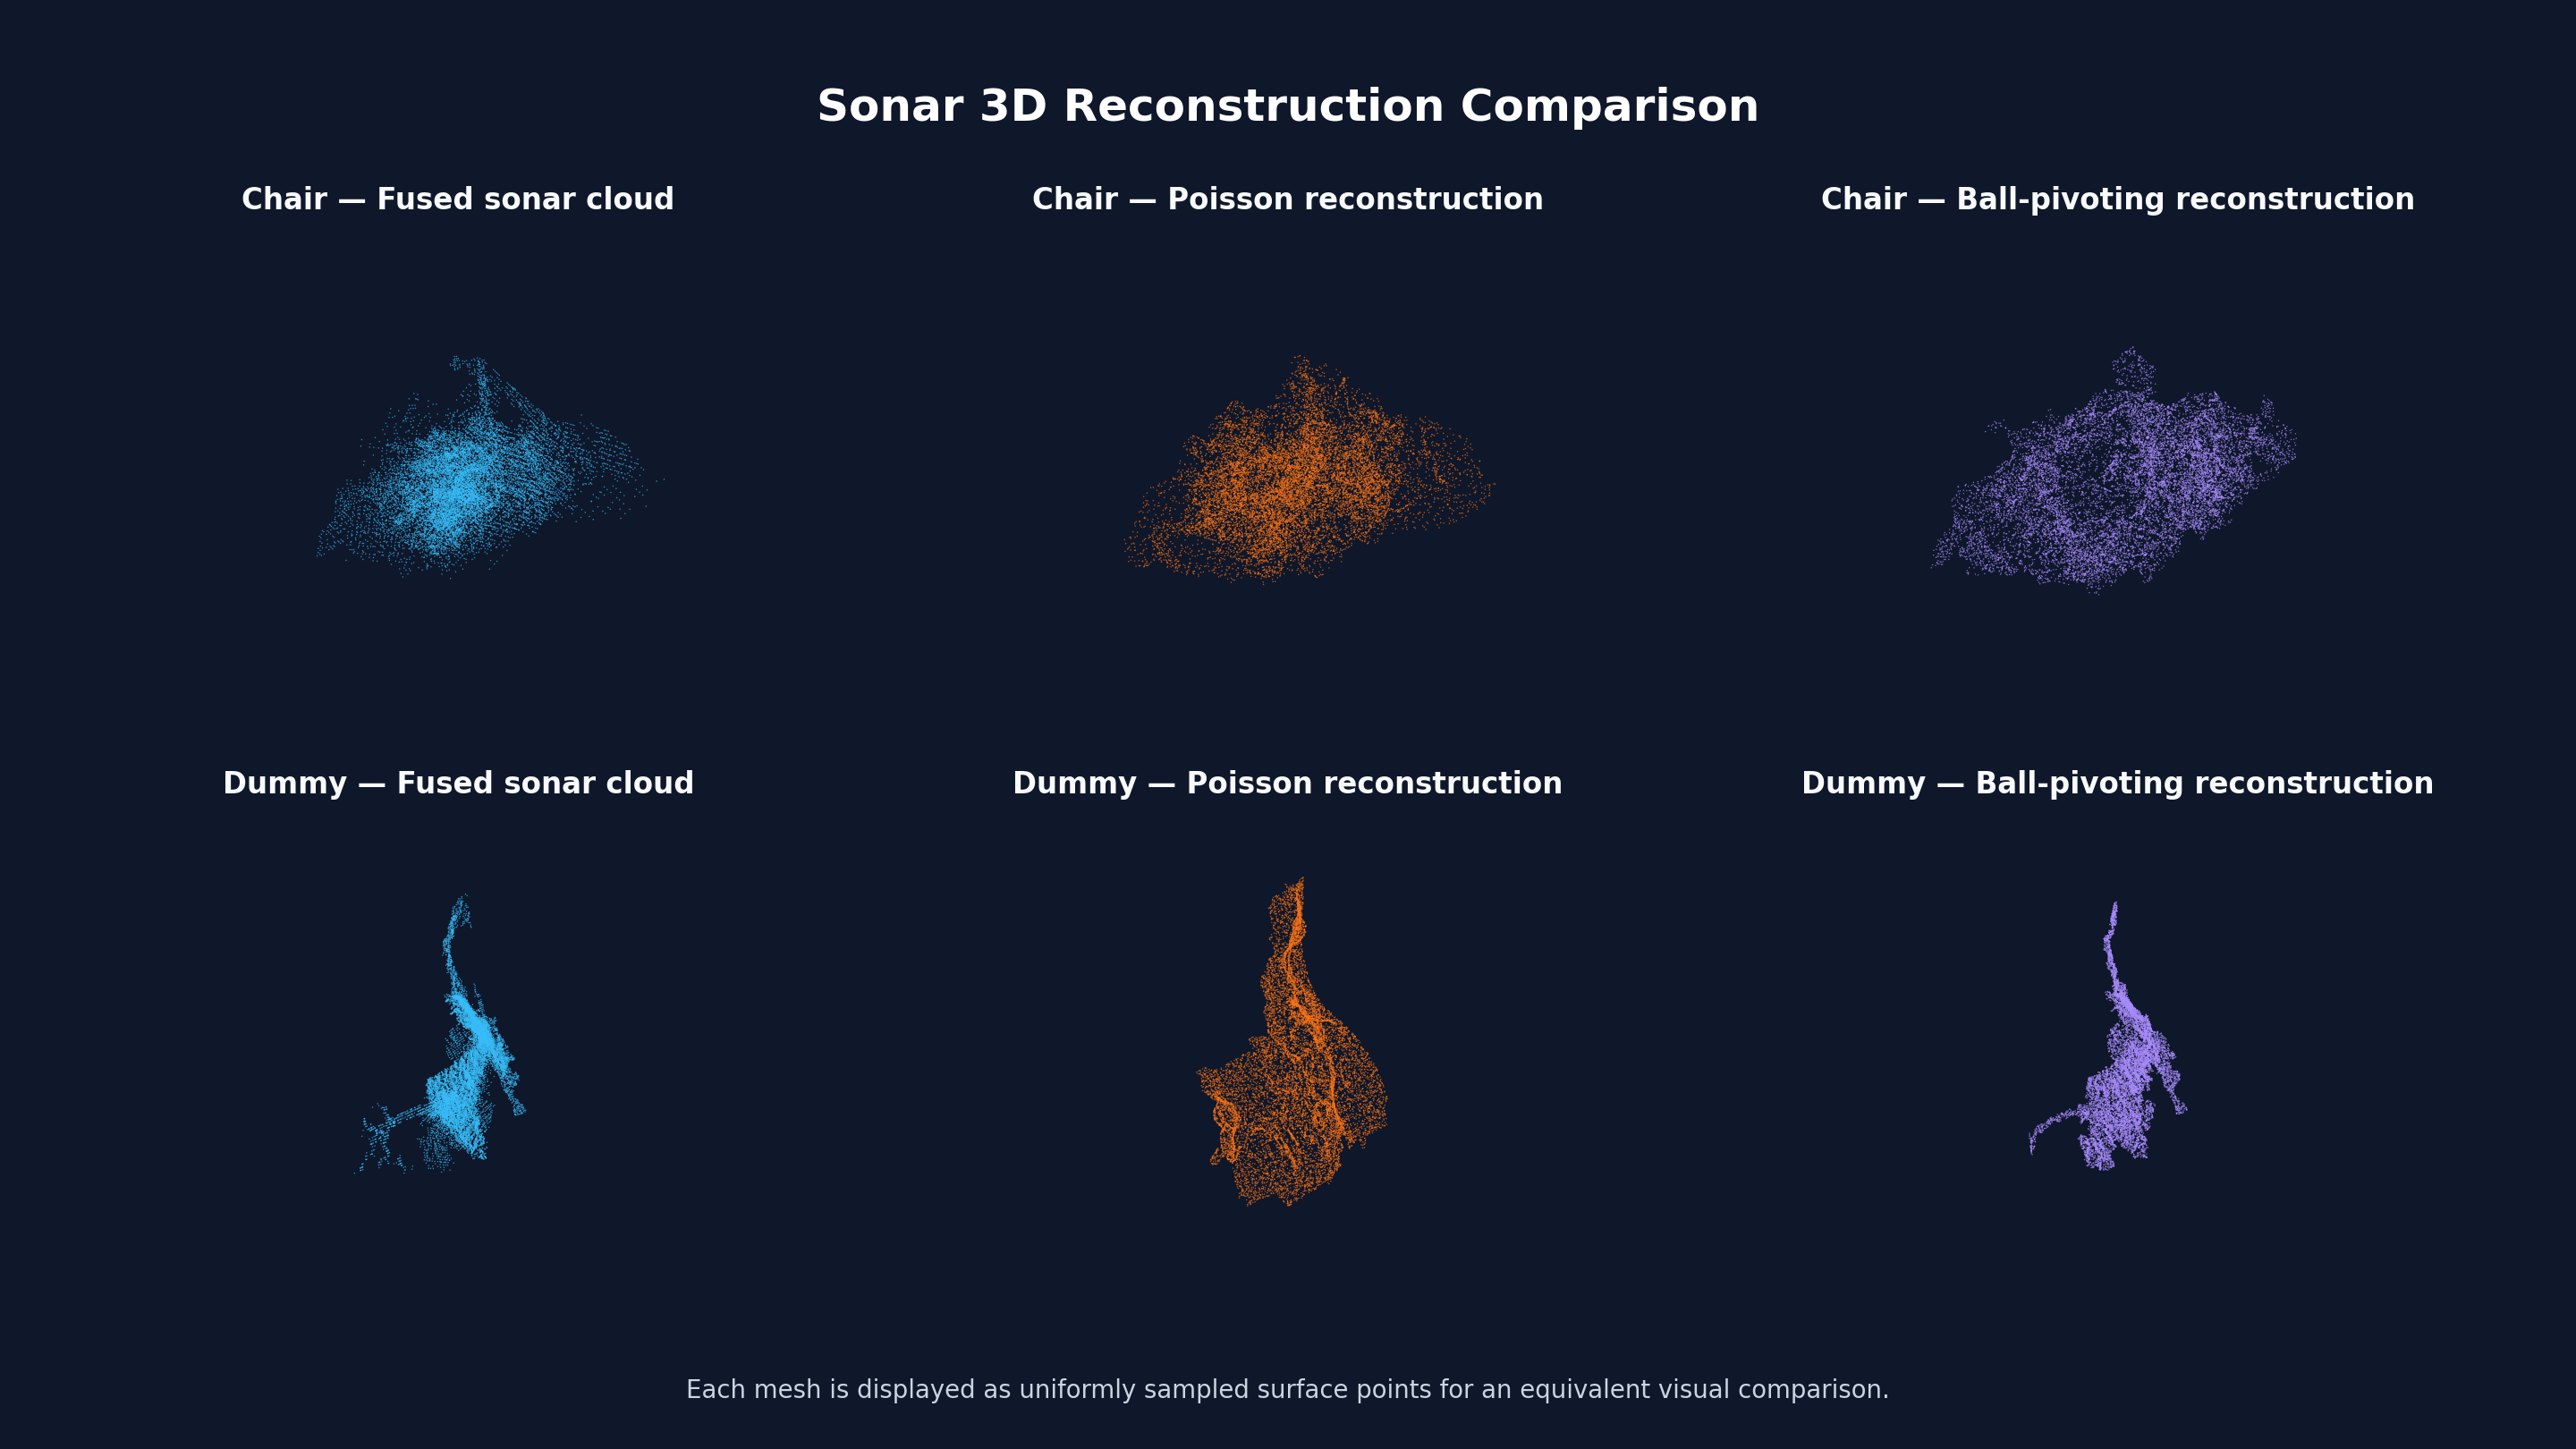
\includegraphics[width=0.92\textwidth]{fig_routeA_comparison.png}
  \caption{Route~A output for the chair and dummy: fused measured cloud,
  Screened Poisson surface and BPA surface rendered together. The two meshers
  expose the trade-off between global smooth completion (Poisson) and local
  evidence-driven triangulation (BPA).}
  \label{fig:routeA_overview}
\end{figure}

\section{Stage 1: pairwise registration}
\label{sec:routea_pairwise}

\subsection{Preprocessing}
Each segmented cloud is translated so its centroid is at the origin, voxel
downsampled at 15~mm (\texttt{VOXEL\_SIZE}), and given normals estimated with a
hybrid search radius of 45~mm (3~$\times$ voxel). Downsampling serves two
purposes: it reduces the cost of the $\binom{n}{2}$ pairwise evaluations, and
it equalises density between views so that fitness values are comparable.
Normals are required by both the FPFH descriptor and the point-to-plane ICP
refinement.

\subsection{FPFH descriptors}
For each downsampled point, FPFH \citep{rusu2009fast} is computed with a
feature radius of 75~mm (5~$\times$ voxel) and up to 100 neighbours. The
descriptor is a 33-dimensional histogram of relative angle features between
the query point and its neighbours. FPFH is chosen because it is fast, robust
to noise, and adequate for the mostly-smooth objects in \suop{}. Its known
weakness --- confusion between \emph{repeated parts} such as chair legs or
tyre treads --- is exactly why pairwise matches are treated as evidence in a
globally optimised graph rather than accepted as truth.

\subsection{RANSAC global alignment}
For every pair $(i,j)$, an initial alignment is sought with RANSAC feature
matching \citep{fischler1981ransac}: candidate correspondences are sampled from
the FPFH matches, the implied rigid transform is computed, and geometrically
consistent inliers are counted under a correspondence distance of 30~mm
(2~$\times$ voxel). The transform with the most inliers (subject to an
edge-length consistency check and a distance check) is returned. RANSAC is
needed because the \suop{} cases share no common frame and ICP alone cannot
converge from an arbitrary initialisation.

\subsection{Point-to-plane ICP refinement}
The RANSAC transform initialises ICP \citep{besl1992method}, which minimises
the point-to-plane distance between corresponding points,
\begin{equation}
\label{eq:icp}
\min_{T} \sum_{(p,q)\in \mathcal{C}(T)}
\big( (T p - q)\cdot n_q \big)^2,
\end{equation}
where $\mathcal{C}(T)$ is the nearest-neighbour correspondence set under $T$ and
$n_q$ is the normal at the target point. The result is scored by its
\emph{fitness} (fraction of inliers) and \emph{inlier RMSE}. The information
matrix for the edge is computed from the inlier correspondences; it is needed
by the pose-graph optimiser to weight the constraint.

\subsection{Edge acceptance}
Only pairwise registrations whose fitness is at least
\texttt{MIN\_FITNESS\_FOR\_EDGE} $= 0.25$ become pose-graph edges. This
threshold is deliberately conservative: a low-fitness registration typically
aligns only a small (often symmetric) subset of the geometry and would inject
false constraints into the graph. The threshold also encodes the observation
that \suop{} scans at 6 and 10~m ranges simply cannot reach fitness 0.25 (their
fitness is typically $<0.1$ after ICP), which is why only 3~m cases are fused.

\section{Stage 2: pose-graph optimisation}
\label{sec:routea_graph}

\subsection{Maximum-fitness spanning tree}
With $n$ views, the pairwise stage yields up to $\binom{n}{2}$ candidate
edges. A \emph{maximum-fitness spanning tree} is built with Prim's algorithm
\citep{cormen2009introduction} over the accepted edges: starting from a
reference view (index 0), the highest-fitness edge connecting the visited set
to an unvisited view is added until all reachable views are connected. The MST
provides two things: (i)~an \emph{initial pose} for every view (composed along
the tree from the reference), and (ii)~a set of \emph{odometry edges} that are
declared certain in the graph.

\subsection{Loop closures}
Every \emph{other} accepted pairwise edge is a \emph{loop-closure} edge,
declared \emph{uncertain} in the graph. Loop closures are what make multiway
fusion better than a naive pairwise chain: they constrain the accumulated
drift by tying non-neighbouring views together. For 24 views, the MST uses 23
edges and the number of loop closures is typically in the tens to hundreds
(\secref{ch:resultsA}).

\subsection{Global optimisation}
The pose graph is optimised with Open3D's global optimisation
\citep{choi2015robust,zhou2018open3d}: a Levenberg--Marquardt solver minimises
the weighted squared residuals over all edges,
\begin{equation}
\label{eq:posegraph}
\min_{\{T_i\}} \sum_{(i,j)\in E}
\left\lVert \log\!\left( T_{ij}^{-1} T_i^{-1} T_j \right) \right\rVert^2_{\Sigma_{ij}},
\end{equation}
where the norm is the weighted geodesic error on $SE(3)$ and $\Sigma_{ij}$ is
the edge information matrix. An edge-pruning threshold of 0.25 removes
outlier constraints during optimisation. The optimised node poses are the
final per-view object poses in the canonical frame.

\section{Stage 3: fusion}
\label{sec:routea_fusion}

Each original (non-downsampled) segment is transformed by its optimised pose
and accumulated into a single point cloud. The fused cloud is voxel
downsampled at half the pairwise voxel (7.5~mm) to produce the final
\emph{measured} representation of the object. The fused cloud is both an
output in its own right and the input to meshing.

\section{Stage 4: surface reconstruction}
\label{sec:routea_meshing}

Two independent meshers are run on the fused, normal-oriented cloud, exposing
complementary behaviours:

\subsection{Screened Poisson reconstruction}
The cloud's normals are oriented consistently
(\emph{orient\_normals\_consistent\_tangent\_plane}), and Screened Poisson
reconstruction \citep{kazhdan2006poisson,kazhdan2013screened} is solved at
octree depth 8. The output is trimmed by removing the 2\% lowest-density
vertices (a standard guard against extrapolation into unsupported space) and
cleaned: degenerate/duplicate triangles, duplicate vertices and non-manifold
edges are removed, and only the largest connected component is kept.
Poisson's strength is a smooth, closed surface that bridges small sampling
gaps; its limitation is that it \emph{will} close large unsupported gaps too,
inflating sparse regions.

\subsection{Ball-Pivoting Algorithm}
BPA \citep{bernardini1999ball} rolls a ball over the cloud with four radii
($1.5, 2, 3, 4$ $\times$ the mean nearest-neighbour distance), creating a
triangle whenever the ball touches three points without enclosing another.
The same cleaning procedure is applied. BPA's strength is that it preserves
genuine gaps (holes remain where sampling is too sparse); its limitation is
that it cannot bridge gaps at all.

\subsection{Why produce both?}
Producing both meshes is not redundancy: it is the honest way to present the
uncertainty of the fusion. Where Poisson and BPA agree, the surface is well
supported by measurements; where they disagree (Poisson fills, BPA is open),
the surface is extrapolated and should be treated as less certain. This
two-mesh discipline is carried into the results and discussion
(\secref{ch:resultsA}, \secref{ch:discussion}).

\section{Variants}
\label{sec:routea_variants}

Two further Route~A variants address the specific weakness of the generic
pipeline on sparse \suop{} evidence: the generic pipeline registers in full
$SE(3)$, which is fragile when segments contain only a few hundred points.

\subsection{View-aware seabed-plane registration}
The view-aware variant (\texttt{reconstruct\_viewaware.py}) exploits the
physical constraint that the object moves \emph{on the seabed plane}. For each
case it: range-gates the 3~m cloud to the shell band $1.75$--$4.0$~m; removes
the seabed plane (RANSAC, 16~mm threshold); keeps only elevated returns
($3.5$--$48$~cm for the chair, $1.5$--$42$~cm for the tyre) that cannot belong
to the seabed; and clusters at the published object scale (chair diagonal
$0.18$--$0.62$~m; tyre $0.38$--$0.92$~m). Acceptable clusters are registered
with an \emph{SE(2)} transform in the seabed plane --- yaw plus planar
translation --- which also moves the sonar origin into the canonical object
frame, and view-oriented surfels are fused with screened Poisson. The
\emph{acceptance} criterion is explicit: a case is accepted only if its planar
fit has an inlier fraction above threshold and a trimmed RMSE below threshold
(e.g.\ $\le 26$~mm). \tabref{tab:routeA_metrics} in \secref{ch:resultsA} reports
the accepted case counts and the surface-fit metrics.

\subsection{Sonar-native first-return ray TSDF}
\label{sec:routea_tsdf}
The sonar-native variant (\texttt{reconstruct\_suop\_tsdf.py}) deliberately
contains no CAD, primitive or learned prior. It treats every registered return
as the first hit on an acoustic ray anchored at the sonar origin: space
\emph{before} the return is free, and a short band \emph{behind} it is
occupied. These signed-distance observations are fused in a dense TSDF
\citep{curless1996volumetric} (4~mm voxels, 18~mm truncation) and the
zero-crossing is extracted with marching cubes \citep{lorensen1987marching}.
Crucially, the mesh is coloured by \emph{measured-return support} and any
vertex without nearby measured support (beyond a 16~mm support limit) is
removed, so unobserved regions cannot masquerade as accurate geometry. This
variant is the most conservative and the most honest about what a single
acoustic return can prove; its results appear in \secref{sec:resultsA_variants}.

\section{Summary}
\label{sec:routea_summary}

\routeA{} is chosen when several scans of a rigid object exist and the output
must be a faithful fusion of measurements. It estimates poses from geometry
(FPFH/RANSAC/ICP), refines them jointly in a pose graph with loop closures,
fuses the aligned measurements and surfaces the result with two complementary
meshers. Two variants harden the pipeline for sparse sonar evidence: a
seabed-plane-constrained SE(2) registration, and a sonar-native first-return
ray TSDF that reports measurement support explicitly. The next chapter
presents the alternative route, which drops the multi-view requirement
entirely and replaces geometry with a learned prior.

% =====================================================================
% Chapter 5 — Route B: Single-View Learned Completion
% =====================================================================
\chapter{Route~B: Single-View Learned Completion}
\label{ch:routeB}

This chapter presents the methodology of \routeB, the learned route. As in the
previous chapter it first justifies \emph{why} Route~B is the appropriate
answer in this project (\secref{sec:why_routeB}), then details the pipeline in
its stages: single-view capture and sonar-realistic simulation
(\secref{sec:routeB_sim}), the PCN architecture (\secref{sec:routeB_arch}),
the construction of paired training data (\secref{sec:routeB_data}), and the
training procedure (\secref{sec:routeB_training}).

\section{Why Route~B?}
\label{sec:why_routeB}

Route~B is the answer to the research question under the following conditions:

\begin{enumerate}
  \item \textbf{Only one partial view is available (or will be at
  deployment).} The \suop{} acquisition protocol moved the object between
  cases without logging its pose, so the multi-view assumption of \routeA{}
  is not always satisfiable. In many operational settings --- a single sonar
  pass over an object, a towed sonar that sees an object once --- only one
  partial observation will ever exist. No geometric fusion can recover the
  occluded side of a single scan, so the only route to a \emph{complete}
  representation is a learned prior.
  \item \textbf{The output must be a complete object representation.}
  Route~A deliberately leaves unobserved regions empty; \routeB{} deliberately
  fills them. Applications that need a full shape --- e.g.\ a matching target
  for a manipulation system, a CAD-like model for simulation, or a
  classification feature --- prefer a complete, prior-informed output over a
  partial but strictly measured one.
  \item \textbf{A shape prior can be obtained.} Because the objects are
  manufactured or quasi-rigid (folding chairs, tyres, drums, mannequins,
  nets), their complete geometry is learnable: procedural parametric models and
  the project's own \routeA{} meshes provide paired training targets
  (\secref{sec:routeB_data}).
\end{enumerate}

The \emph{core assumption} of Route~B is that a network trained on many
(partial, complete) pairs learns a prior $p(\text{complete}\mid\text{partial})$
over the shape category, so that at inference a single partial cloud can be
mapped to a complete point set. Route~B is therefore a conditional-generation
problem: encode the partial view, decode a complete cloud, and supervise with a
symmetric distance to a reference. The route's pipeline is summarised in
\figref{fig:routeB_overview}.

\begin{figure}[H]
  \centering
  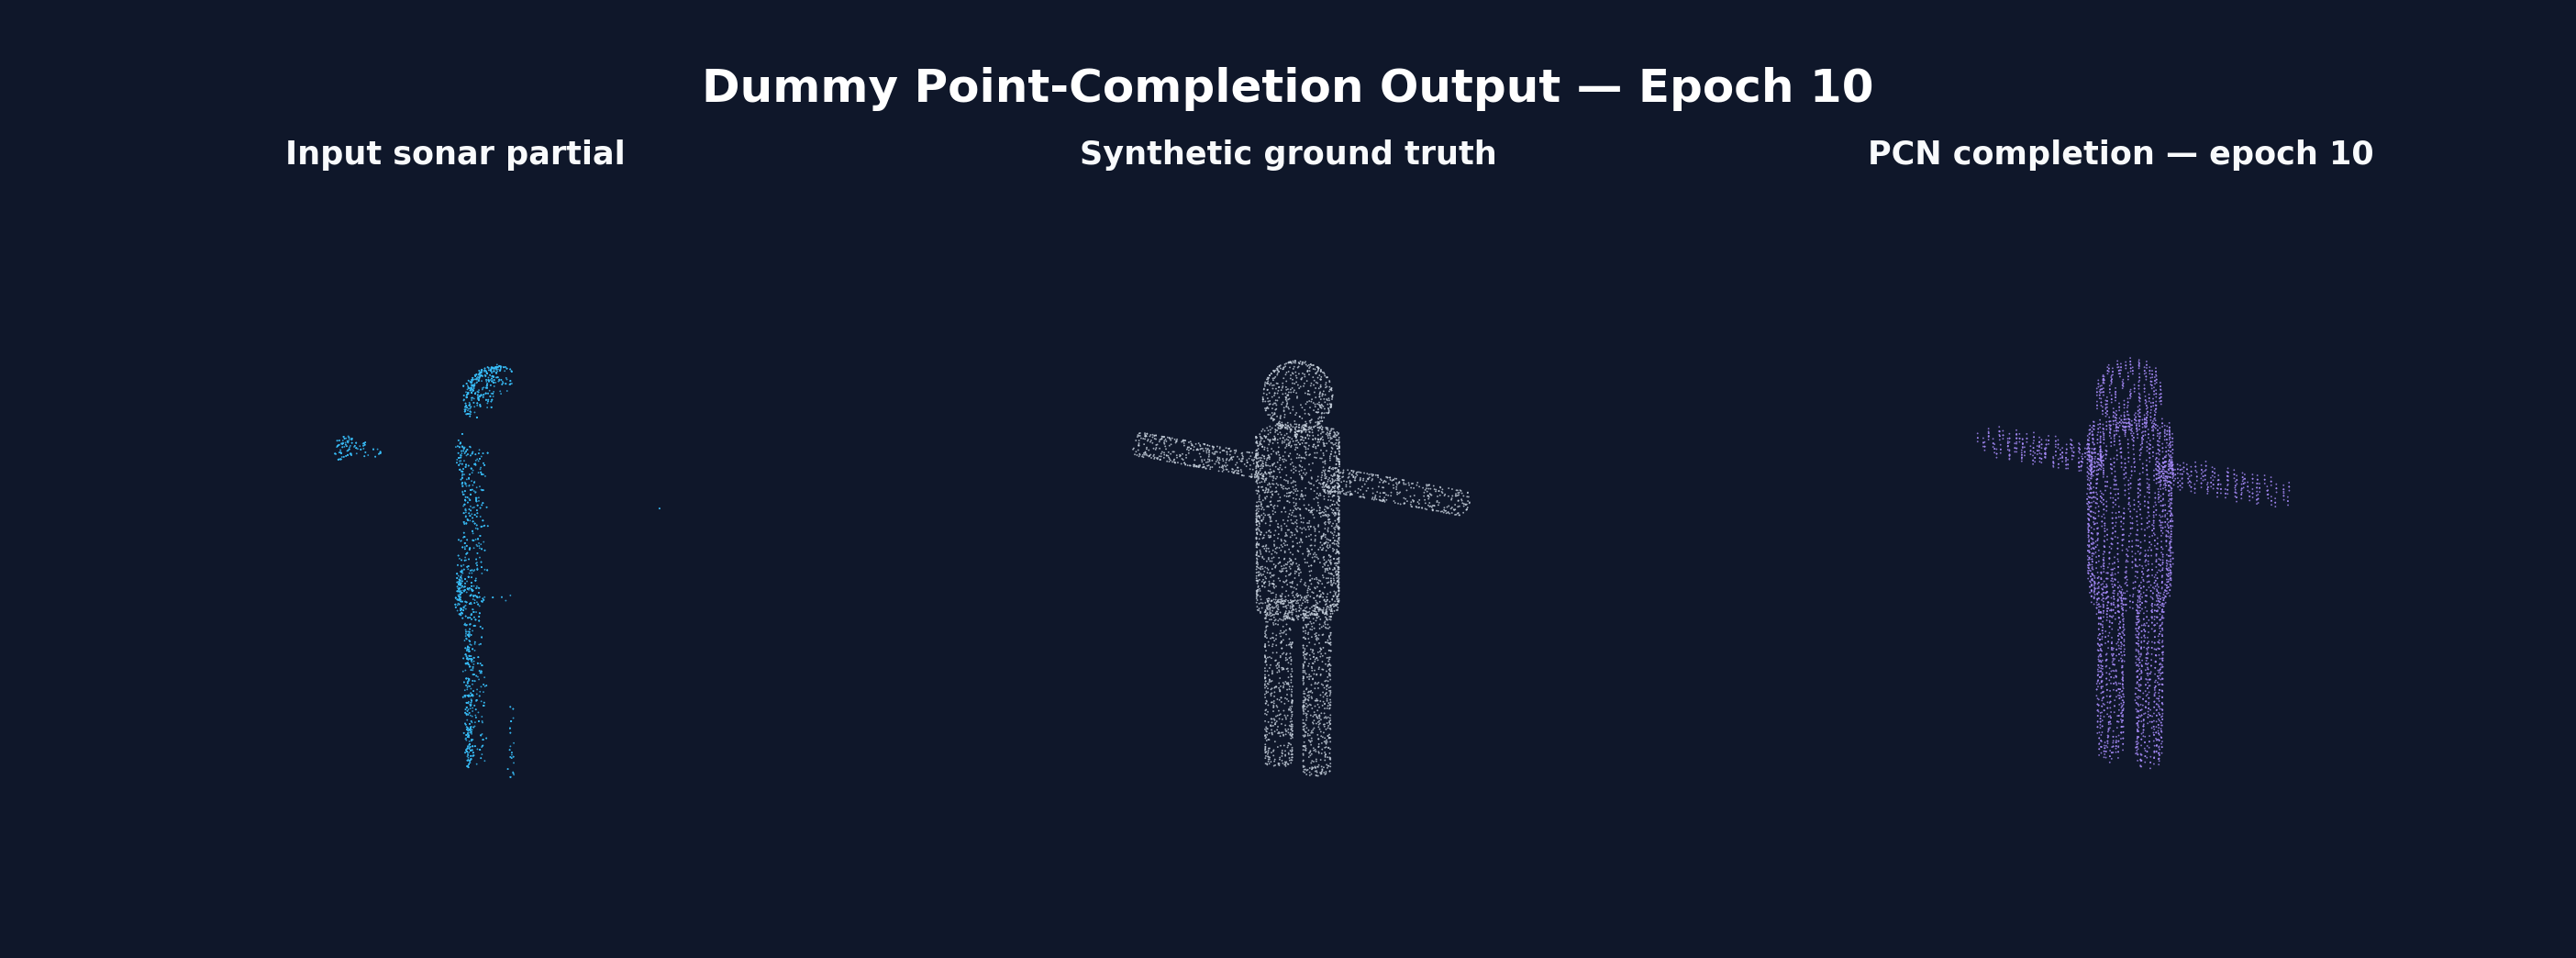
\includegraphics[width=0.9\textwidth]{fig_routeB_dummy.png}
  \caption{Route~B output for the dummy after 10 epochs: left, the sonar-like
  partial input; centre, the complete reference used as ground truth; right,
  the PCN fine completion. The completion contains inferred points in regions
  that were never visible in the input.}
  \label{fig:routeB_overview}
\end{figure}

\section{Stage 1: single-view capture and simulation}
\label{sec:routeB_sim}

\subsection{Real capture}
At inference, the input to \routeB{} is a single segmented sonar partial
cloud. In this project the real \suop{} chair segment shown in
\figref{fig:chair_pcn} is used directly: a single case's segmented returns are
normalised to the PCN input size of 2048 points and fed to the trained network
without any multi-view processing.

\begin{figure}[H]
  \centering
  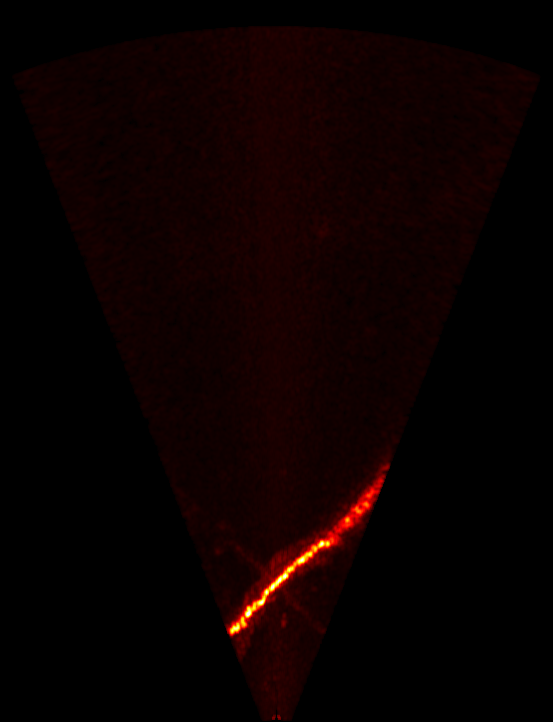
\includegraphics[width=0.55\textwidth]{fig_chair_ping.png}
  \caption{A single real \suop{} chair ping (fan-shaped range return). A
  single view of this kind is the deployment input for \routeB{}: the object's
  far side, underside and much of its frame are simply absent from the data.}
  \label{fig:chair_pcn}
\end{figure}

\subsection{Simulated acquisition}
Because \suop{} contains no (partial, complete) ground-truth pairs, training
partials are generated from complete references. For every training sample the
following pipeline is applied (\texttt{simulate\_sonar\_partial} in
\texttt{train\_pcn.py}):

\begin{enumerate}
  \item \textbf{Viewpoint sampling.} A virtual camera is placed at a random
  azimuth $\phi \in [0, 2\pi)$ and elevation $\psi \in [-0.3, 0.6]$~rad at a
  distance of $2.5$--$4.0$ $\times$ the object diameter, i.e.\ representative of
  a 3~m-range sonar look at the published object scales.
  \item \textbf{Hidden-point removal.} Open3D's
  \texttt{hidden\_point\_removal} \citep{katz2007direct} keeps exactly the
  subset of the complete surface visible from that viewpoint, mimicking
  acoustic shadowing: the far side of the object is removed.
  \item \textbf{Sonar degradation.} Gaussian range noise with standard
  deviation $6$--$15$~mm is added to simulate beam/range error, and with
  probability $0.5$ a contiguous angular sector (span $0.5$--$1.5$~rad) is
  removed, imitating an occlusion shadow behind a strong return.
  \item \textbf{Resampling.} The resulting partial is (sub- or over-)sampled to
  exactly 2048 points, the PCN input size.
\end{enumerate}

The partial is normalised using the \emph{full shape} frame (centre and max
norm of the complete reference), so that the partial and the ground truth share
a common scale --- this is essential, because the Chamfer loss is
scale-sensitive. \figref{fig:sim_partial} illustrates the simulation.

\begin{figure}[H]
  \centering
  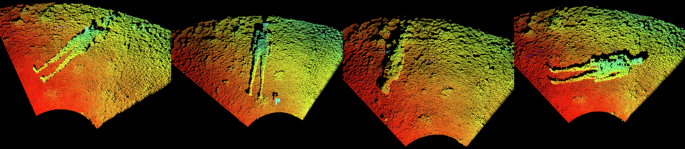
\includegraphics[width=0.9\textwidth]{fig_sim_partial.png}
  \caption{Sonar-realistic partial simulation. A complete reference shape is
  viewed from a random viewpoint (hidden-point removal keeps only visible
  points), then corrupted with Gaussian range noise and an angular sector
  removal that imitates an acoustic shadow.}
  \label{fig:sim_partial}
\end{figure}

\section{Stage 2: the PCN architecture}
\label{sec:routeB_arch}

The network is the Point Completion Network \citep{yuan2018pcn}, implemented
from scratch in PyTorch \citep{paszke2019pytorch}. Its design is summarised in
\tabref{tab:pcn_arch}.

\begin{table}[H]
  \centering
  \small
  \begin{adjustbox}{max width=\textwidth}
  \begin{tabular}{@{}llll@{}}
    \toprule
    Block & Operation & Output size & Notes \\
    \midrule
    Input & --- & $N \times 3$ & $N = 2048$ partial points \\
    Encoder MLP 1 & Conv1d($3\to128\to256$), ReLU & $256 \times N$ & shared per point \\
    Max pool (local) & \texttt{max} over points & $256 \times 1$ & PointNet symmetry \\
    Encoder MLP 2 & Conv1d($512\to512\to1024$), ReLU & $1024 \times N$ & concat with pooled \\
    Max pool (global) & \texttt{max} over points & $1024$ & global latent $\mathbf{v}$ \\
    FC decoder & Linear($1024\!\to\!1024\!\to\!1024\!\to\!3M$) & $M \times 3$ & coarse, $M = 1024$ \\
    Folding decoder & Conv1d($1024{+}2{+}3 \to 512 \to 3$) & $M g^2 \times 3$ & fine, $g \in \{2,4\}$ \\
    \bottomrule
  \end{tabular}
  \end{adjustbox}
  \caption{\pcn{} architecture used in this project. The encoder is a
  PointNet-style shared-MLP plus symmetric max pooling that produces a
  permutation-invariant 1024-dimensional global latent; the decoder predicts
  $M$ coarse points with a fully connected head and then folds a $g\times g$
  grid around each coarse point to produce $M g^2$ fine points.}
  \label{tab:pcn_arch}
\end{table}

\subsection{Encoder: why shared MLPs and max pooling}
Points are unordered, so any encoder must be \emph{permutation invariant}.
Shared MLPs applied per point (implemented as $1\times1$ convolutions) give a
feature for every point; the symmetric max pooling operation then aggregates
the strongest learned response per channel into a global feature that does not
depend on the order of the input points. The second MLP block sees the
concatenation of per-point features and the pooled feature, which gives each
point local context before the final pooling step. The output is a single
1024-dimensional vector summarising the partial shape.

\subsection{Decoder: why coarse-to-fine with folding}
Decoding 4096 structured points from one vector is a difficult regression. The
coarse-to-fine strategy splits it: a fully connected head predicts $M=1024$
coarse points that capture the global skeleton (seat, legs, rim, barrel, etc.);
each coarse point then \emph{sprouts} a $g\times g$ grid of fine points via
the folding operation
\begin{equation}
  \mathbf{f}_{i,k} \;=\; \mathbf{c}_i \;+\;
  \mathrm{MLP}\big( [\,\mathbf{c}_i;\; \mathbf{u}_{i,k};\; \mathbf{v}\,]\big),
  \qquad \mathbf{u}_{i,k} \in [-0.05,\;0.05]^2 ,
  \label{eq:folding}
\end{equation}
where a per-point MLP maps the
concatenation of the coarse point, the grid coordinate and the global latent to
a small offset. Folding lets the network refine local detail while remaining
tied to the global latent, which is why it is preferred over a second fully
connected head \citep{yang2018folding,yuan2018pcn}. With $g=2$ the fine cloud
has 4096 points; with $g=4$, 16{,}384 points. The output is a point cloud,
never a mesh.

\section{Stage 3: paired training data}
\label{sec:routeB_data}

\subsection{Two generators}
\label{sec:routeB_generators}
Complete reference clouds come from two generators:

\begin{enumerate}
  \item \textbf{Generator 1 --- procedural parametric models.}
  \texttt{make\_chair}, \texttt{make\_tire}, \texttt{make\_drum} and
  \texttt{make\_dummy} in \texttt{train\_pcn.py} build Open3D meshes from
  randomised dimensions matched to the published \suop{} nominal sizes: a
  folding chair from boxes (seat $0.40$--$0.50$~m, backrest, four legs
  $0.03$--$0.05$~m thick), a tyre from a torus ($R = 0.28$--$0.34$~m,
  $r = 0.08$--$0.13$~m), a drum from a cylinder (radius $0.26$--$0.34$~m,
  height $1.0$--$1.3$~m), and a dummy mannequin from a torso cylinder, head
  sphere, and limb cylinders with randomised proportions. Each mesh is sampled
  uniformly to 8192 surface points.
  \item \textbf{Generator 2 --- mesh-conditioned on \routeA{} output.}
  \texttt{gen\_suop\_dummy\_dataset.py} builds training pairs from the
  \emph{actual reconstructed \routeA{} meshes} (e.g.\ \texttt{meshes/dummy\_bpa.ply}):
  it samples 100{,}000 surface points from the mesh, then for each sample
  applies a random yaw rotation and a $\pm4\%$ scale jitter before running the
  partial simulation of \secref{sec:routeB_sim}. This deliberately links the
  two routes: the learned completion prior is conditioned on the geometry that
  the geometric route actually recovered from sonar, rather than on an ideal
  CAD shape.
\end{enumerate}

\subsection{Output pairs}
Each training sample is a pair $(\mathbf{P}, \mathbf{G})$: a 2048-point
sonar-like partial cloud and a 4096-point complete reference, both normalised
to the unit sphere in the full-shape frame. Datasets were generated with
$n = 6000$ pairs (e.g.\ \texttt{dataset\_dummy\_suop.npz},
\texttt{dataset\_drum\_suop.npz}) using a multiprocessing pool, in a few
minutes on eight cores. A 10\% hold-out provides validation.

\section{Stage 4: training}
\label{sec:routeB_training}

\subsection{Loss}
The training objective is the symmetric Chamfer distance
\eqref{eq:chamfer} applied to both the coarse and the fine predictions,
\begin{equation}
  L \;=\; \mathrm{CD}(C, G) \;+\; \mathrm{CD}(F, G),
  \label{eq:routeB_loss}
\end{equation}
where $C$ and $F$ are the coarse and fine outputs. As explained in
\secref{sec:lit_completion}, the symmetric form combines an accuracy term
(predictions must be near the reference) with a completeness term (every
reference point must be covered), preventing collapse to a small safe subset.

\subsection{Optimiser and schedule}
Training uses Adam \citep{kingma2015adam} with learning rate $10^{-3}$ and
batch size 32--48; a StepLR scheduler halves the learning rate every 40 epochs.
All data are preloaded onto the GPU once to avoid per-batch host transfers. On
an NVIDIA RTX~4060 Laptop GPU (8~GB), ten epochs of 6000 pairs take roughly
26--28 minutes. Checkpoints are saved per epoch (for contact sheets) and as a
final \texttt{.pth} file.

\subsection{Training runs}
\label{sec:routeB_runs}
Four training runs were executed:

\begin{itemize}
  \item \texttt{pcn\_dummy\_suop\_10ep.pth} --- dummy, mesh-conditioned
  (Generator~2), 10 epochs;
  \item \texttt{pcn\_drum\_suop\_10ep.pth} --- drum, Generator~1, 10 epochs;
  \item \texttt{pcn\_chair.pth} --- chair, Generator~1, 150 epochs
  (the long run that produced the epoch-1-to-15 progression of
  \figref{fig:chair_pcn_progression});
  \item \texttt{pcn\_dummy\_10ep.pth} / \texttt{pcn\_dummy\_5ep.pth} ---
  exploratory dummy runs used to tune the simulation and grid size.
\end{itemize}

The training progress of the dummy and drum runs is shown in
\figref{fig:dummy_epochs} and \figref{fig:drum_epochs}; the corresponding loss
curves are reported in \secref{ch:resultsB}.

\section{Summary}
\label{sec:routeB_summary}

\routeB{} is chosen when only one view exists and a complete representation is
required. It simulates sonar-like partials from complete references, encodes a
partial with a PointNet-style architecture, and decodes a coarse-to-fine
completion with a folding network, trained end-to-end with a symmetric Chamfer
loss. Its training targets come from procedural models and --- uniquely ---
from the project's own \routeA{} meshes, creating a principled bridge between
the two routes. The next chapter compares the two routes directly and makes
the difference in their outputs explicit.

% =====================================================================
% Chapter 6 — Why Route A, Why Route B: The Two Routes Compared
% =====================================================================
\chapter{Why \routeA, Why \routeB: The Two Routes Compared}
\label{ch:comparison}

This chapter is the conceptual core of the dissertation. \secref{ch:routeA}
and \secref{ch:routeB} each justified their own route; this chapter
\emph{contrasts} them directly so that the choice is explicit and the
difference in output meaning is unmistakable. It first positions the two
routes as different answers to the same question under different data
availability (\secref{sec:cmp_positioning}), then compares them side by side
on motivation, assumptions, input requirements, ground truth and evaluation
(\secref{sec:cmp_table}), and finally discusses the \emph{output differences}
in depth (\secref{sec:cmp_outputs}).

\section{Positioning: two routes, one question}
\label{sec:cmp_positioning}

The research question of \secref{sec:research_question} --- how to turn
incomplete sonar returns into a useful 3D representation --- admits two
fundamentally different answers, and which one is \emph{correct} depends on
data availability and on what the output will be used for. The two routes are
\emph{complementary, not interchangeable}:

\begin{quote}
\routeA{} is the right answer \emph{when several scans of a rigid object
exist} and the output must be a \emph{fusion of measurements}: it estimates
poses, aligns the scans, and surfaces the measured evidence. \routeB{} is the
right answer \emph{when only one view exists} and a \emph{complete} object
representation is needed: it encodes the partial and decodes the missing
geometry from a learned prior.
\end{quote}

This is why the project implements both: neither route dominates the other,
because they answer different sub-problems of the same question. The decision
procedure is:

\begin{enumerate}
  \item \textbf{How many views of the object are available?} If several
  overlapping views exist and can be aligned, \routeA{} is available and its
  output is strictly more trustworthy (measured). If only one view exists,
  only \routeB{} can produce a complete output.
  \item \textbf{What is the output for?} If the application can tolerate (or
  requires) unmeasured regions, \routeB{}'s completeness is a feature. If the
  application must not be misled by hallucinated geometry (inspection, safety
  assessment), \routeA{}'s honesty is decisive.
  \item \textbf{Is a shape prior available and trusted?} \routeB{} depends on
  the training distribution: it will produce plausible-but-wrong geometry for
  shapes outside that distribution. \routeA{} needs no prior beyond object
  scale.
\end{enumerate}

\section{Side-by-side comparison}
\label{sec:cmp_table}

\tabref{tab:route_comparison} compares the two routes across every dimension
that a reader or examiner might question: motivation, assumption, input,
output, ground truth, failure modes and evaluation.

\begin{table}[H]
  \centering
  \small
  \begin{adjustbox}{max width=\textwidth}
  \begin{tabular}{@{}p{2.9cm}p{5.6cm}p{5.6cm}@{}}
    \toprule
    Dimension & \routeA{} (geometric fusion) & \routeB{} (learned completion) \\
    \midrule
    \textbf{Chosen when} & several scans of the same rigid object exist &
    only one partial view exists (or will exist at deployment) \\
    \textbf{Core assumption} & scans are noisy partials of one rigid object;
    there exist rigid transforms aligning them & training pairs teach a prior
    over complete object geometry; a complete reference exists for training \\
    \textbf{Input} & $N$ segmented 3~m scans (24 curated per object) &
    one segmented partial cloud (2048 points) \\
    \textbf{Internal operations} & FPFH $\to$ RANSAC $\to$ ICP $\to$ pose graph
    (MST + loop closures) $\to$ fusion $\to$ Poisson/BPA (or ray TSDF) &
    PointNet-style encoder $\to$ global latent $\to$ coarse head $\to$ folding
    decoder \\
    \textbf{Output} & fused measured cloud + two meshes; vertices with no
    measurement support are removed & coarse + fine completed point clouds;
    unobserved regions are inferred \\
    \textbf{Output meaning} & \emph{what was measured}, aligned and fused &
    \emph{what was inferred}, guided by a learned prior \\
    \textbf{Ground truth} & none external: the scans themselves are the
    evidence (no CAD mesh, no logged pose in \suop{}) & complete reference
    cloud paired with each partial (procedural or Route~A-mesh-derived) \\
    \textbf{Typical failure} & registration error propagates through the
    graph; symmetric parts confuse FPFH; sparse regions over- or under-filled
    by the mesher & hallucination: plausible-but-wrong geometry outside the
    training distribution; scale errors \\
    \textbf{Evaluation metric} & registration fitness/RMSE, graph
    connectivity, fused-point counts, mesh statistics, measured-to-surface
    residual & Chamfer distance (accuracy + completeness), visual
    partial/reference/completion comparison \\
    \textbf{Do not compare with} & \chd{} loss of \routeB{} & mesh counts of
    \routeA{} \\
    \bottomrule
  \end{tabular}
  \end{adjustbox}
  \caption{Direct comparison of the two routes. The critical column is
  ``Output meaning'': \routeA{} fuses measurements, \routeB{} infers missing
  geometry. Consequently their evaluation metrics measure different questions
  and must not be exchanged.}
  \label{tab:route_comparison}
\end{table}

\section{Output differences in depth}
\label{sec:cmp_outputs}

\subsection{What each output claims}
The most important intellectual point of this dissertation is that the two
outputs make \emph{different epistemological claims}:

\begin{itemize}
  \item \routeA{} claims: \emph{``every output point is a registered sonar
  return (or a surface interpolated between such returns); where no
  measurements exist, the surface is either left open (BPA) or explicitly
  trimmed (Poisson, ray TSDF).''} The output is an \emph{evidence report}.
  \item \routeB{} claims: \emph{``this is a complete object as predicted by a
  prior learned from the training distribution; some of these points were
  never measured and are inferred.''} The output is a \emph{model hypothesis}.
\end{itemize}

This distinction has three practical consequences.

\paragraph{1. Completeness versus fidelity.}
\routeA{} is typically less complete: parts of the object that no scan saw
remain empty, and the two meshers disagree there (Poisson closes, BPA stays
open). \routeB{} is always complete by construction: the decoder emits the
same fixed number of points regardless of how much of the object was visible.
Completeness is only meaningful relative to the ground truth, which \routeA{}
does not have in \suop{} and \routeB{} does.

\paragraph{2. Ground-truth availability.}
Because \routeA{}'s input is the only evidence, its accuracy cannot be checked
against an external truth in \suop{} --- there is no CAD model and no logged
pose. The honest metrics are therefore internal consistency (fitness, RMSE,
connectivity, fused counts) and measured-to-surface residuals, plus a
claim-free visual comparison. \routeB{} has an explicit paired reference, so
its accuracy \emph{can} be measured --- but only within the training
distribution, and a low Chamfer loss does not imply that the inference is
physically correct (the network may have learned the prior rather than the
specific object).

\paragraph{3. What ``better'' means.}
Because the two outputs answer different questions, a single ``which route is
better?'' is ill-posed. \routeB{}'s Chamfer loss is not comparable with
\routeA{}'s mesh statistics: a large \routeA{} mesh is not better than a small
one, and a small \routeB{} loss on synthetic partials is not evidence that the
geometric route failed. The only meaningful comparison would require a common
reference --- a calibrated acquisition with logged poses and an external scan
of the same objects --- which is exactly the future-work experiment of
\secref{ch:conclusions}.

\section{When the routes connect}
\label{sec:cmp_connection}

Despite their differences, the routes are not isolated. \routeB{}'s
Generator~2 (\secref{sec:routeB_generators}) samples training references from
\routeA{} meshes, so the learned prior is conditioned on what the geometric
route actually recovered from sonar. This creates a virtuous loop: where
\routeA{} has strong evidence, the prior is grounded in measured geometry; and
where \routeB{} then infers a complete shape, it does so from a distribution
that matches the sensor's output rather than an idealised CAD shape. The two
routes are best understood as partners: \routeA{} establishes the measured
core, \routeB{} extrapolates it into a complete model.

\section{Summary}
\label{sec:cmp_summary}

The choice between \routeA{} and \routeB{} is governed by data availability and
output purpose, not by which pipeline is ``more advanced''. \routeA{} answers
``what did we measure?'' with a pose-corrected fusion of the evidence;
\routeB{} answers ``what is the whole object?'' with a prior-informed
completion. Their outputs differ in completeness, in the status of unobserved
regions, and in the availability of ground truth --- and therefore their
evaluation protocols differ too. The next two chapters report the experimental
results of each route in turn.

% =====================================================================
% Chapter 7 — Route A Results
% =====================================================================
\chapter{Route~A Results}
\label{ch:resultsA}

This chapter reports the experimental results of \routeA{}. It presents the
registration outcomes for all five \suop{} categories
(\secref{sec:resultsA_registration}), the mesh statistics
(\secref{sec:resultsA_meshing}), the variant results (view-aware and ray TSDF,
\secref{sec:resultsA_variants}) and a discussion of what the numbers do and do
not prove (\secref{sec:resultsA_interpretation}). The full pipeline ran on all
five object categories with the 24-view curation described in
\secref{ch:dataset}; every run produced fused clouds and both meshes, i.e.\
5/5 categories completed the full geometric pipeline.

\section{Registration results}
\label{sec:resultsA_registration}

\tabref{tab:registration_results} summarises the pose-graph stage for the five
objects. All $24 \times 5$ views were connected: for every category the
maximum-fitness spanning tree reached 24/24 views and no segment was left
outside the graph. The number of reliable pairwise edges (fitness $\geq 0.25$)
varies between 131 (drum) and 197 (dummy) of the 276 pairs tested, and the
number of loop closures --- edges beyond the 23 MST edges --- ranges from 108
to 174. The high loop-closure counts are important: they mean the pose graph
was strongly over-constrained, so drift along the tree was corrected by many
independent constraints rather than trusted as a chain.

\begin{table}[H]
  \centering
  \small
  \begin{adjustbox}{max width=\textwidth}
  \begin{tabular}{@{}lcccccc@{}}
    \toprule
    Object & Views & Reliable edges & MST edges & Loop closures & Fused points (raw) & Fused points (7.5~mm) \\
    \midrule
    Tyre  & 24 & 172 & 23 & 149 & 37{,}031 & 33{,}970 \\
    Dummy & 24 & 197 & 23 & 174 & 22{,}692 & 21{,}421 \\
    Drum  & 24 & 131 & 23 & 108 & 106{,}436 & 99{,}544 \\
    Chair & 24 & 189 & 23 & 166 & 30{,}519 & 26{,}027 \\
    Net   & 24 & 162 & 23 & 139 & 31{,}288 & 28{,}251 \\
    \bottomrule
  \end{tabular}
  \end{adjustbox}
  \caption{Route~A pose-graph results. 276 pairwise registrations were tested
  per object ($\binom{24}{2}$); edges with fitness $\geq 0.25$ entered the
  graph; the maximum-fitness spanning tree used 23 edges and every remaining
  reliable edge became a loop closure. Fused counts are the pose-corrected
  points before and after the 7.5~mm fusion voxel. All 24 views were reachable
  for every object.}
  \label{tab:registration_results}
\end{table}

The pairwise computation cost was substantial but feasible: between 912~s
(dummy) and 1098~s (chair) per object on the CPU for the 276 pairwise
FPFH/RANSAC/ICP evaluations, dominated by the RANSAC global alignment. This is
an offline cost and was accepted; the per-view ICP refinement itself is
milliseconds once initialised.

\begin{figure}[H]
  \centering
  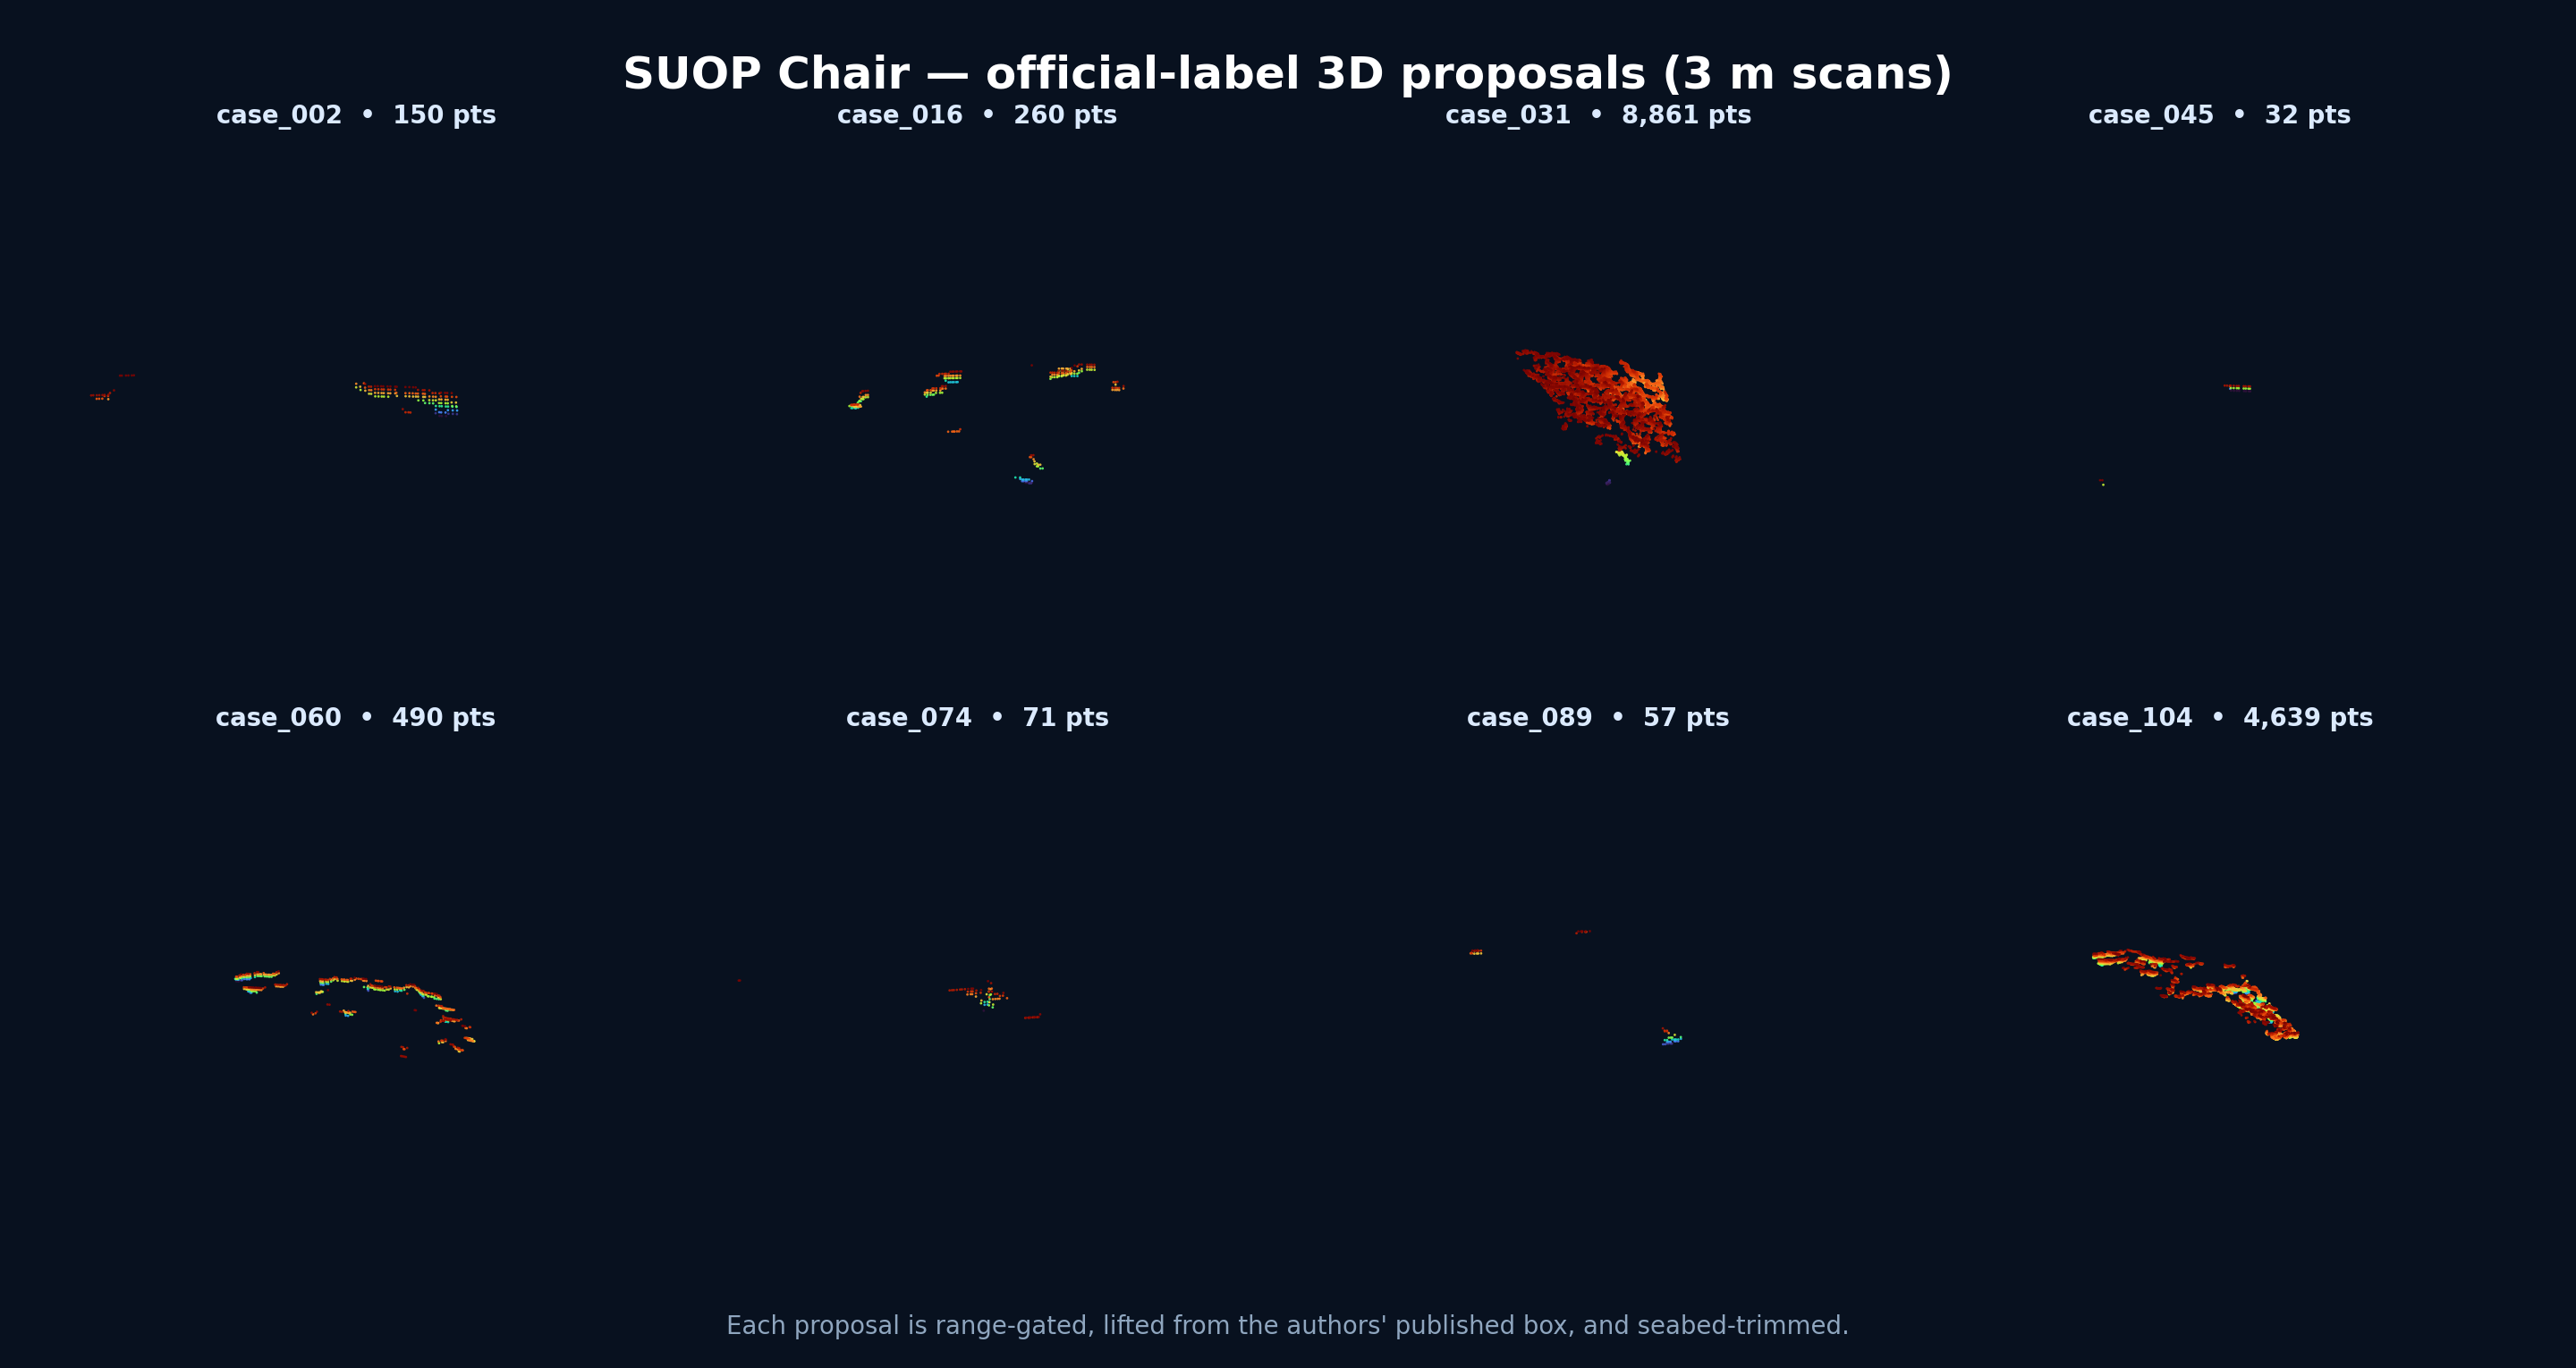
\includegraphics[width=0.92\textwidth]{fig_chair_segments.png}
  \caption{Segmented chair views used as \routeA{} input (one panel per
  accepted case). Each panel shows the isolated chair cluster after seabed-plane
  removal and scale-consistent clustering at the published $0.40$~m diagonal
  scale. The views are partial and noisy --- note the variable leg coverage ---
  yet registration must still align them into one frame.}
  \label{fig:chair_segments}
\end{figure}

\section{Meshing results}
\label{sec:resultsA_meshing}

Both Screened Poisson (depth 8) and BPA (four radii) produced clean meshes for
all five objects. \tabref{tab:meshing_results} reports vertex and triangle
counts after trimming and cleaning (largest connected component only).

\begin{table}[H]
  \centering
  \small
  \begin{adjustbox}{max width=\textwidth}
  \begin{tabular}{@{}lcccccc@{}}
    \toprule
    Object & Fused points & Poisson verts & Poisson tris & BPA verts & BPA tris \\
    \midrule
    Tyre  & 33{,}841 & 69{,}819 & 139{,}684 & 14{,}143 & 24{,}009 \\
    Dummy & 21{,}306 & 29{,}787 & 59{,}419 & 11{,}194 & 19{,}331 \\
    Drum  & 99{,}678 & 125{,}598 & 251{,}677 & 33{,}429 & 53{,}649 \\
    Chair & 25{,}872 & 85{,}891 & 172{,}484 & 9{,}534 & 15{,}317 \\
    Net   & 28{,}240 & 76{,}319 & 152{,}721 & 5{,}220 & 8{,}313 \\
    \bottomrule
  \end{tabular}
  \end{adjustbox}
  \caption{Route~A mesh statistics. Poisson (depth 8, trimmed at the 2\%
  lowest-density vertices) produces smooth closed surfaces with many more
  vertices; BPA produces sparser surfaces that preserve genuine gaps. The
  divergence between the two column pairs is itself the evidence of
  measurement uncertainty (see \secref{sec:resultsA_interpretation}).}
  \label{tab:meshing_results}
\end{table}

\begin{figure}[H]
  \centering
  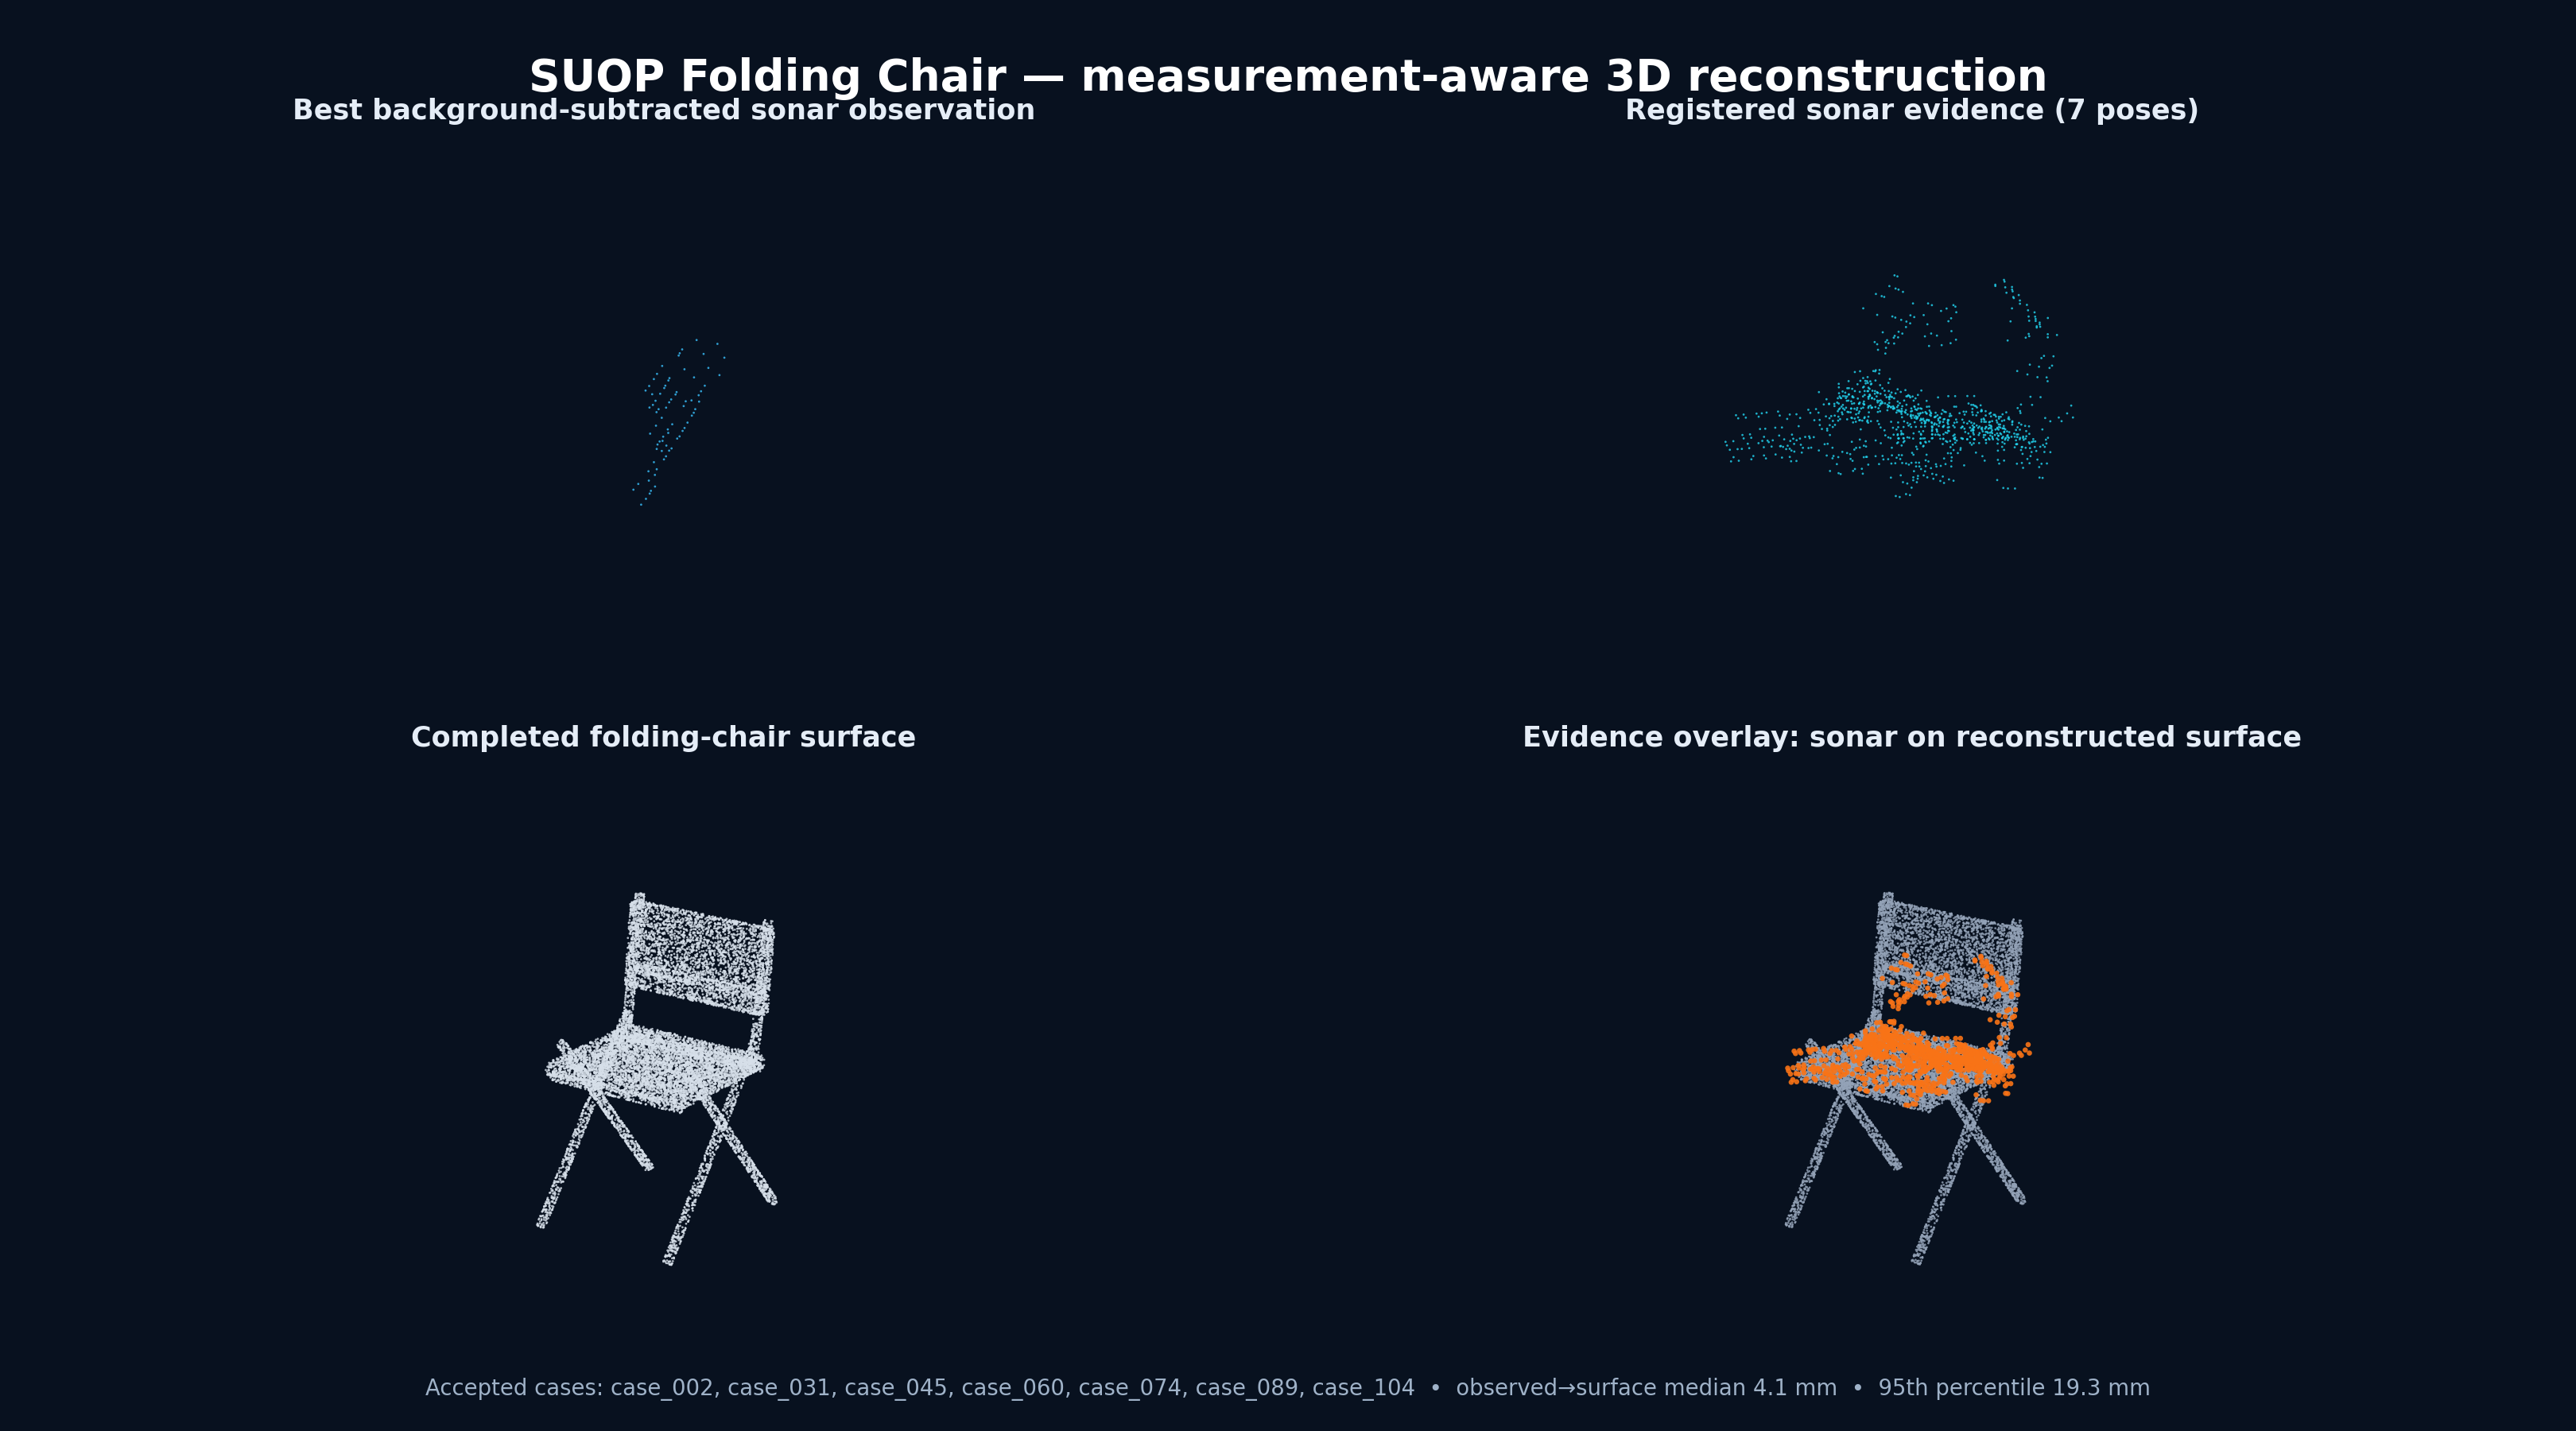
\includegraphics[width=0.94\textwidth]{fig_chair_reconstruction.png}
  \caption{Route~A chair: fused measured cloud and the two meshes. The chair's
  open frame is a stress test: leg-like structures are registered across many
  views, and the difference between the closed Poisson surface and the open BPA
  surface is clearly visible in the seat underside and between legs.}
  \label{fig:chair_reconstruction}
\end{figure}

\begin{figure}[H]
  \centering
  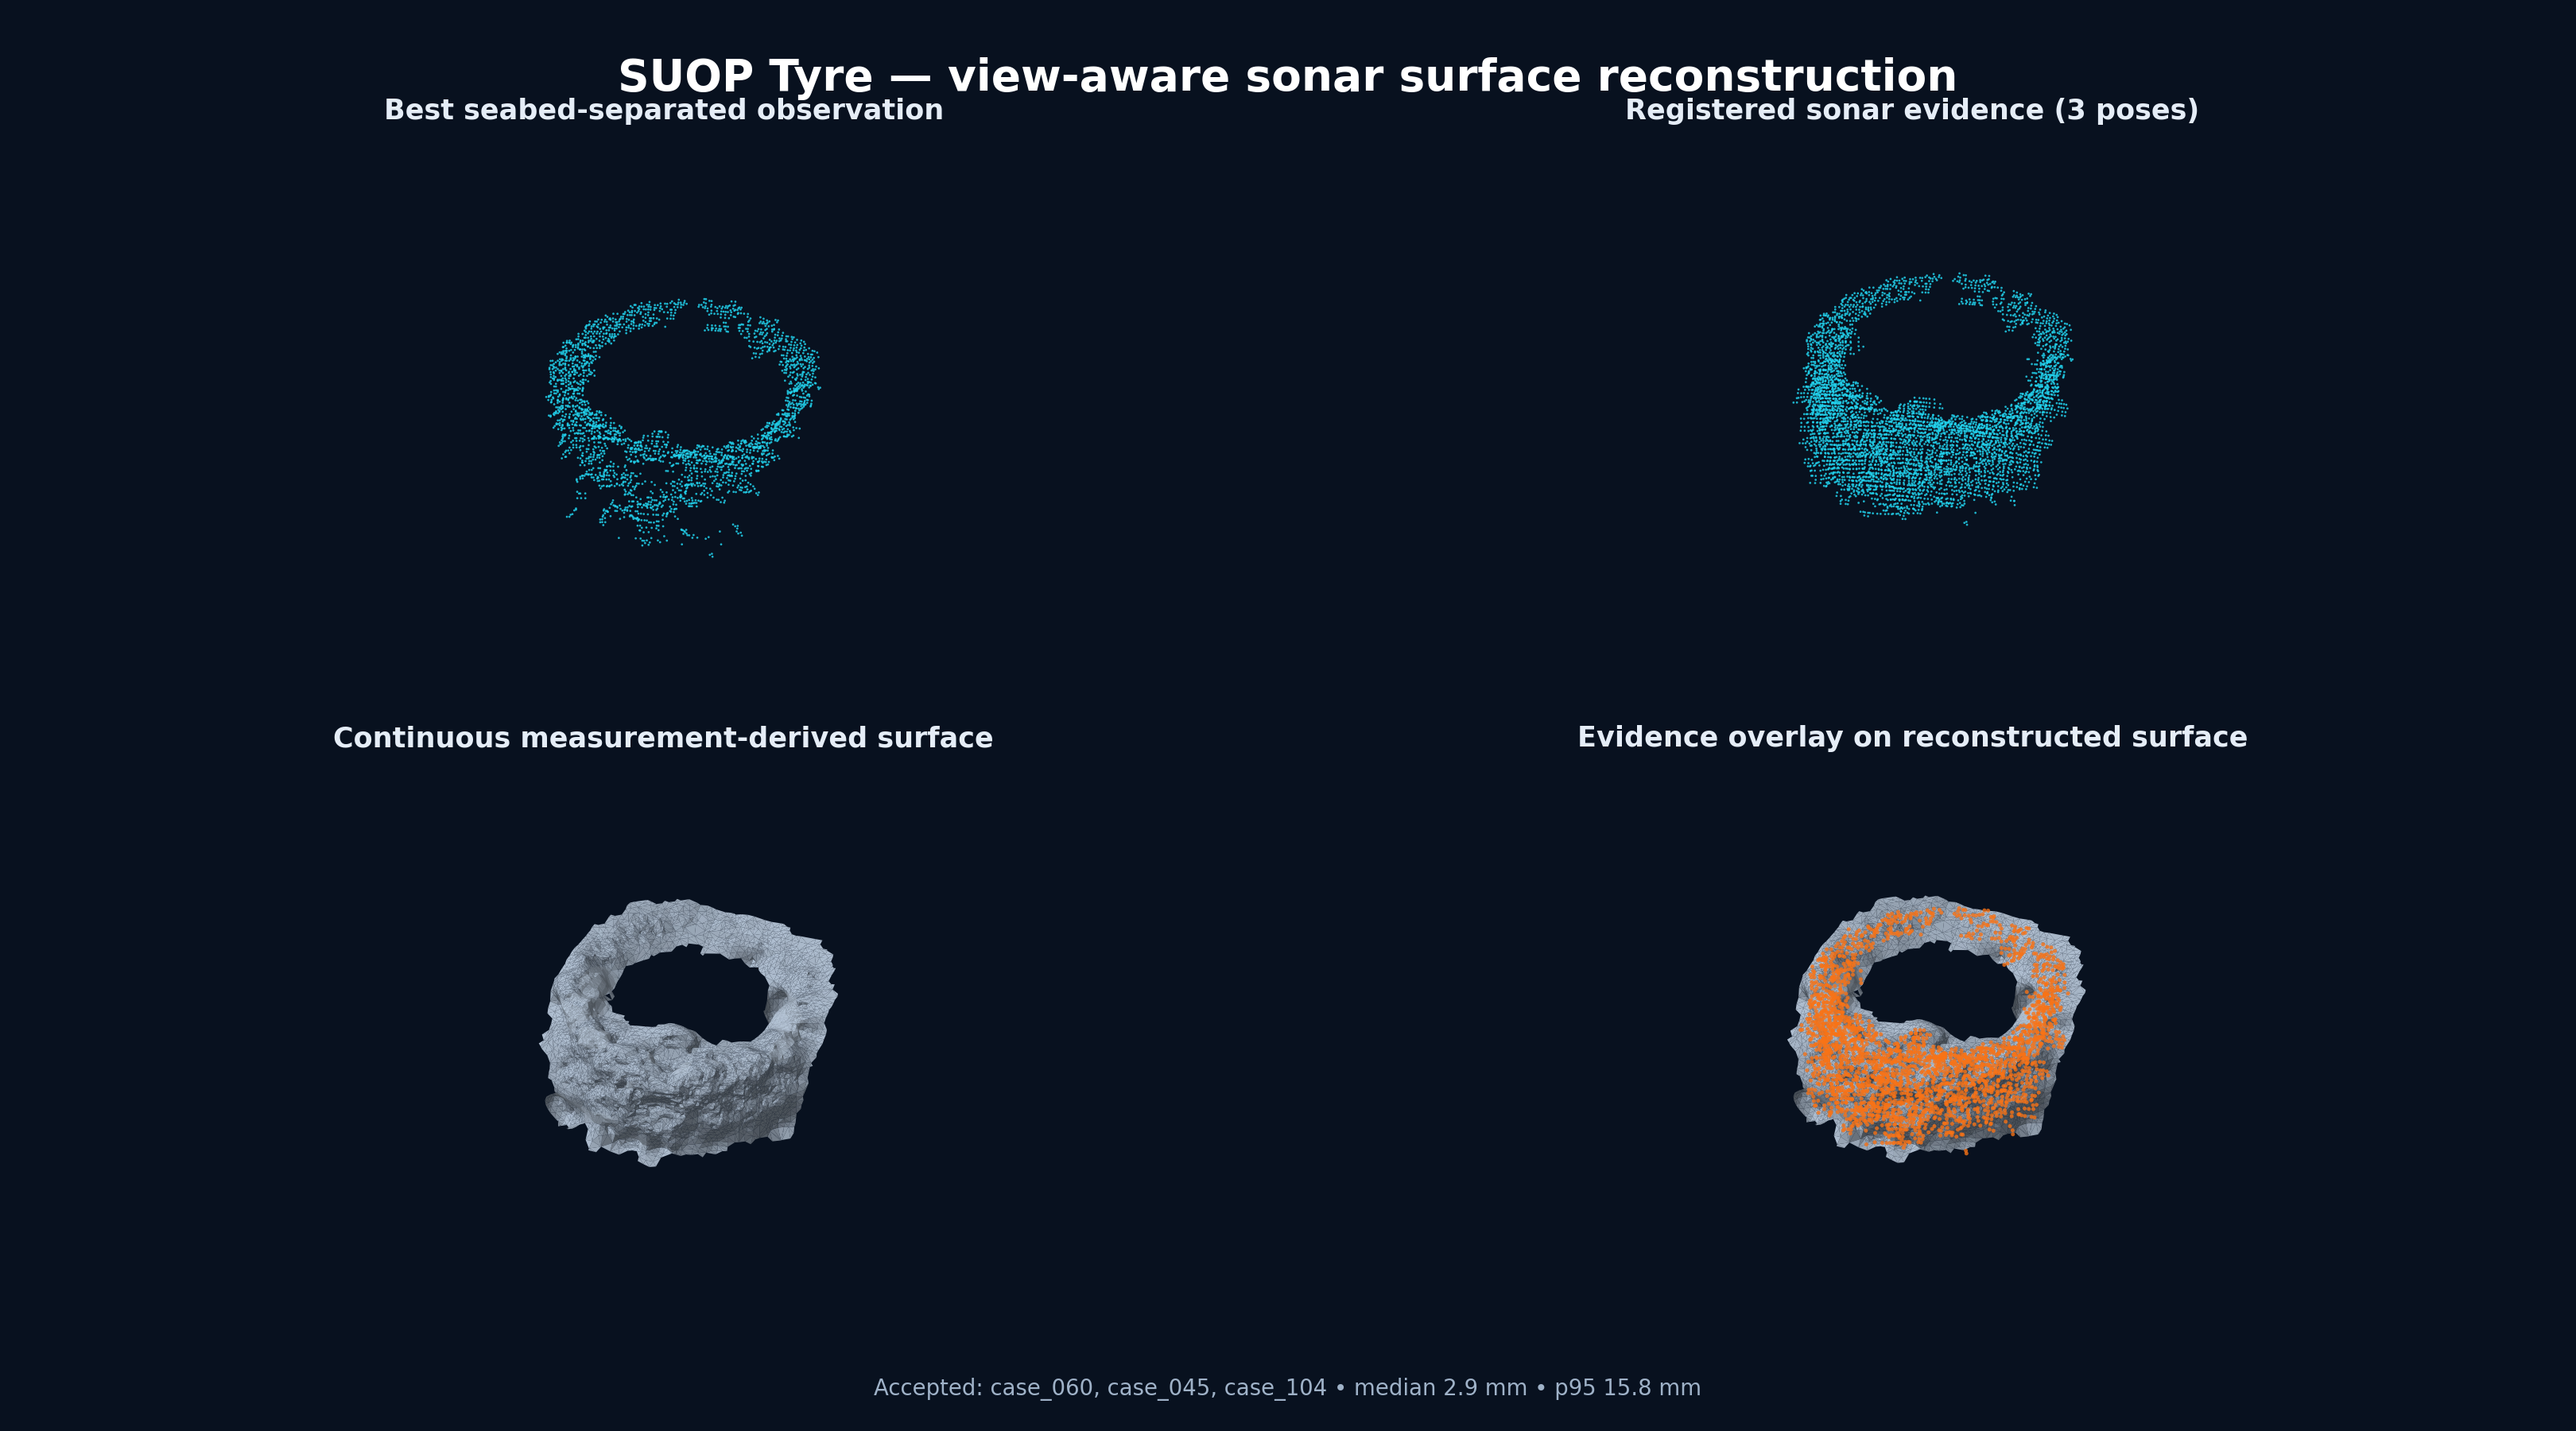
\includegraphics[width=0.94\textwidth]{fig_tyre_reconstruction.png}
  \caption{Route~A tyre: fused cloud, Poisson and BPA surfaces. The toroidal
  rim is recovered; the inner wall and far side, which no 3~m view observed
  fully, show the Poisson-vs-BPA disagreement most clearly.}
  \label{fig:tyre_reconstruction}
\end{figure}

\begin{figure}[H]
  \centering
  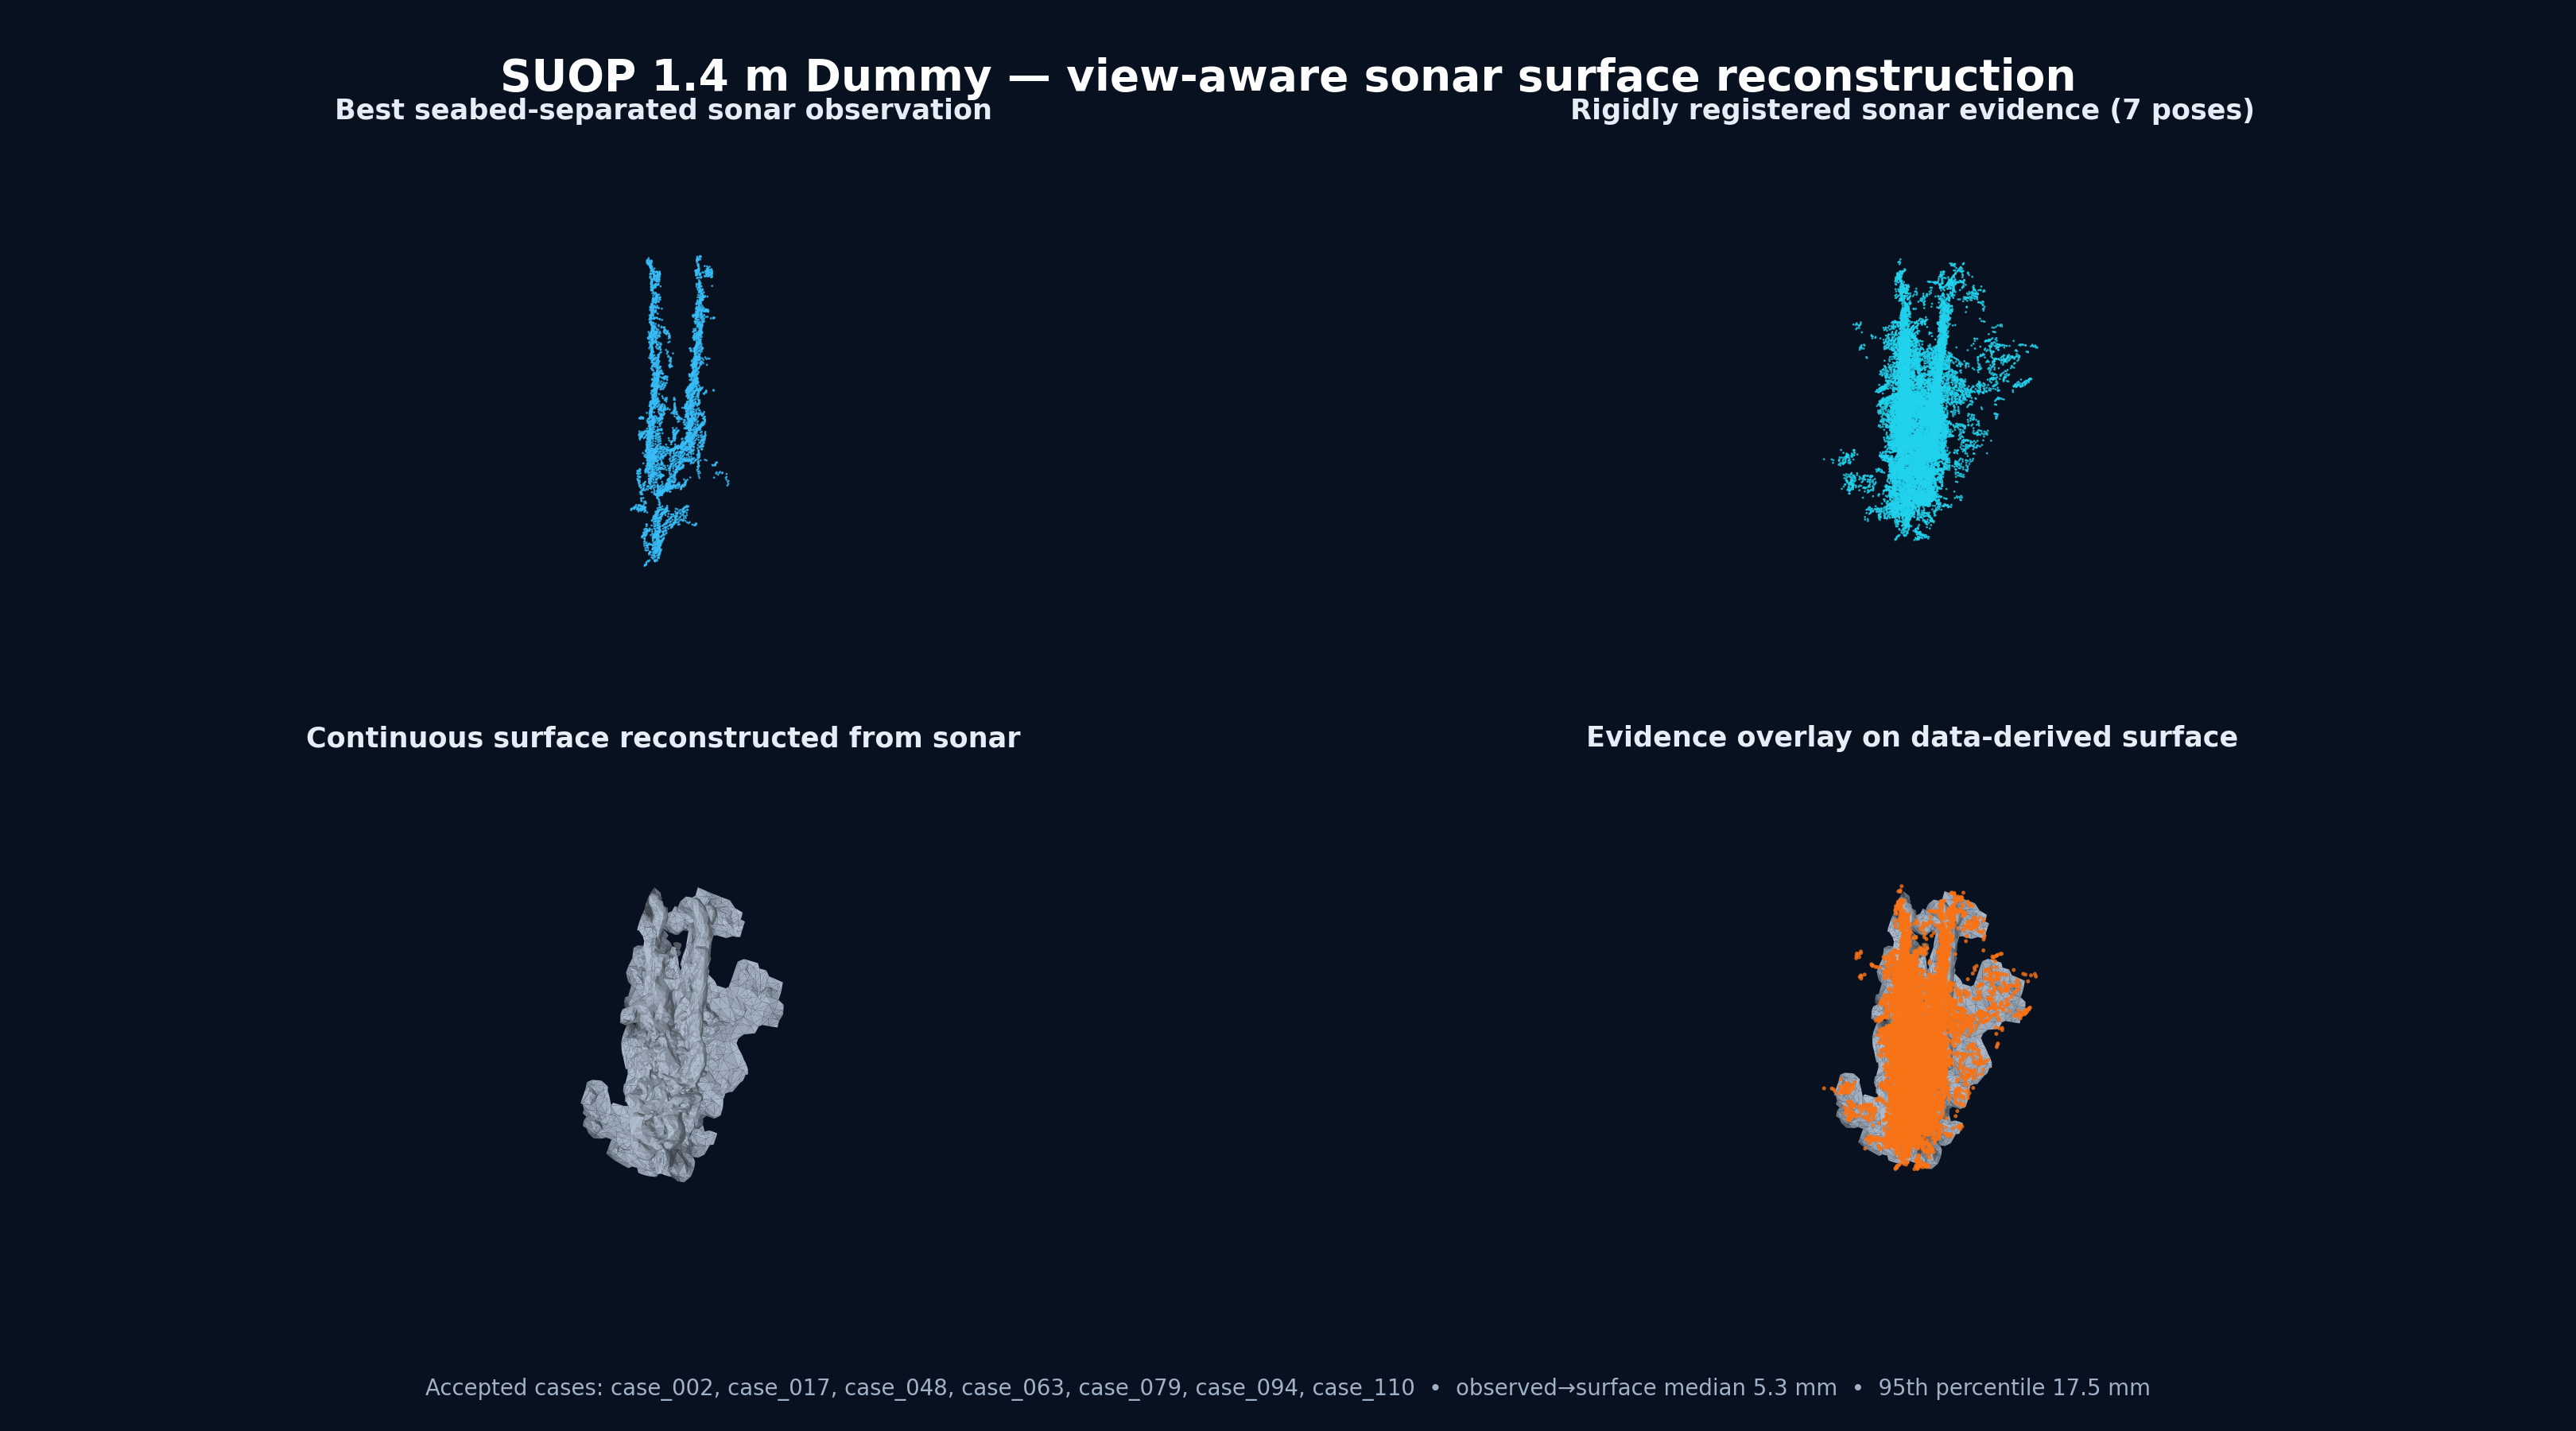
\includegraphics[width=0.94\textwidth]{fig_dummy_reconstruction.png}
  \caption{Route~A dummy: fused cloud, Poisson and BPA surfaces. The vertical
  mannequin shape and the shoulder/arm junctions are visible; the head and
  torso are the best-supported regions.}
  \label{fig:dummy_reconstruction}
\end{figure}

\subsection{Turntable views}
\figref{fig:chair_turntable} shows the chair reconstruction rotated around the
vertical axis. The turntable renders make the 3D consistency of the fused
model auditable from all sides rather than from a single favourable angle.

\begin{figure}[H]
  \centering
  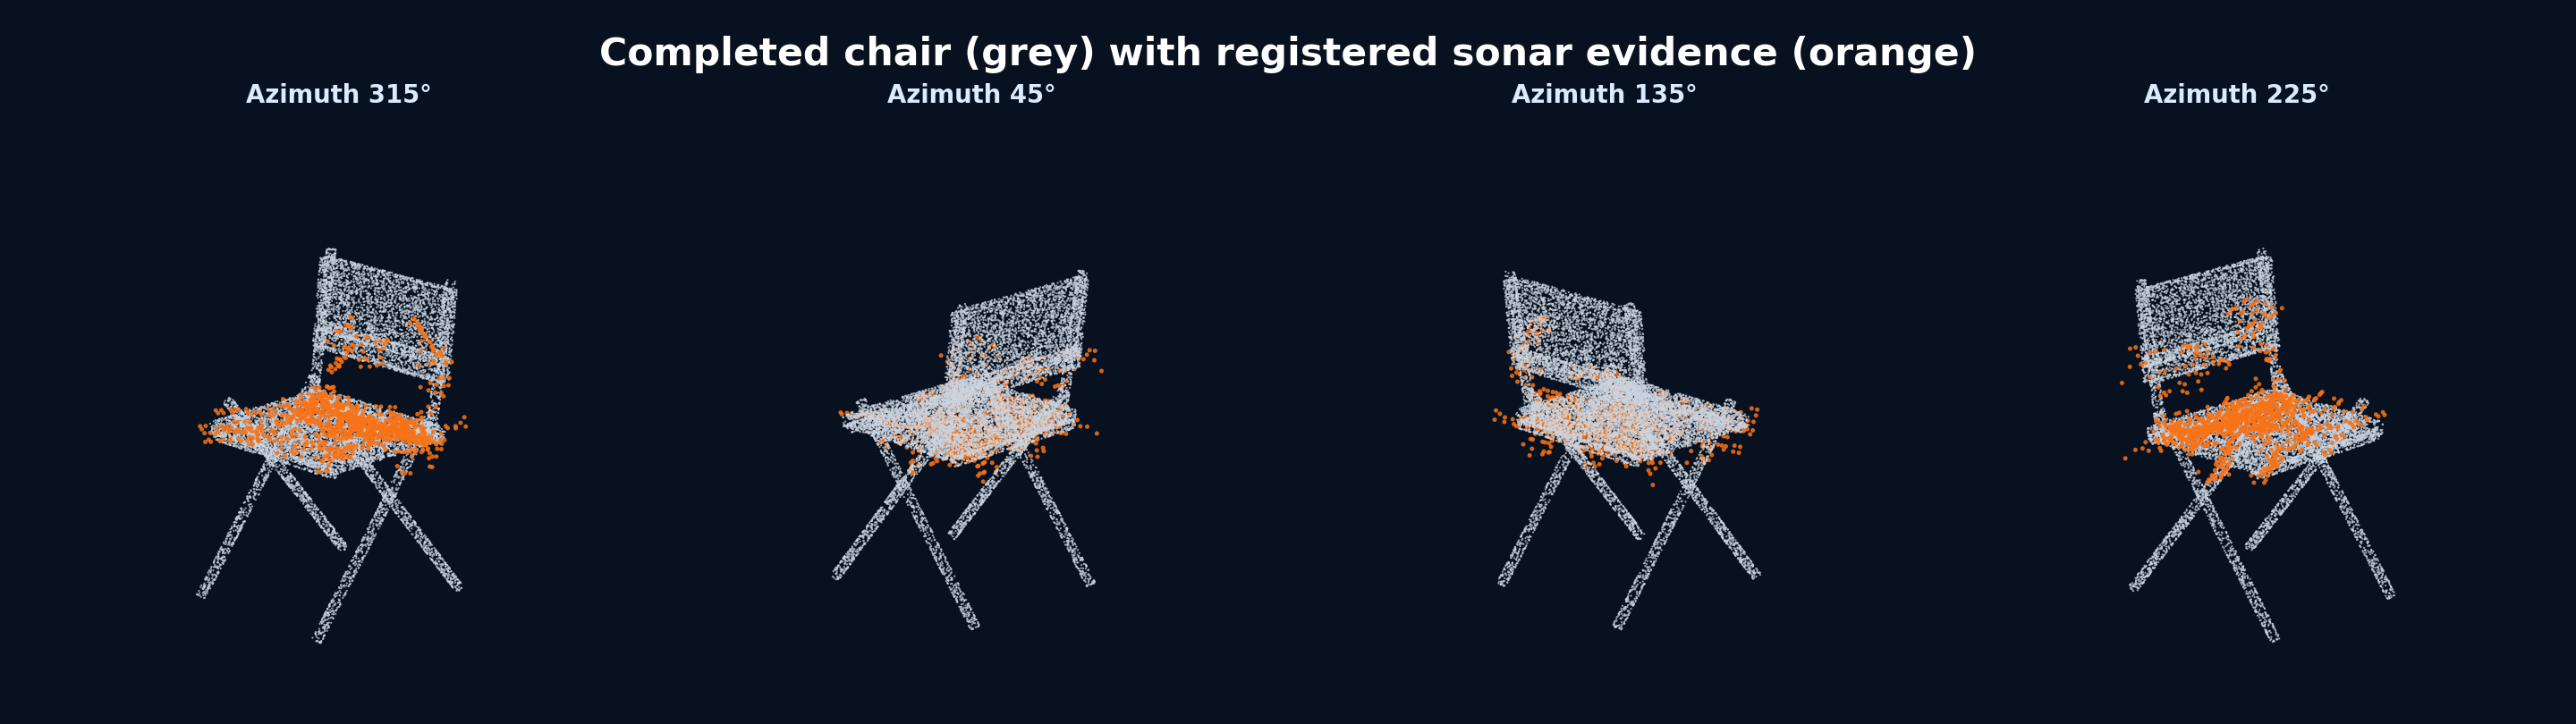
\includegraphics[width=0.98\textwidth]{fig_chair_turntable.png}
  \caption{Chair reconstruction turntable: the same fused model viewed from
  eight azimuths. Consistency across views is the visual equivalent of the
  graph's loop-closure redundancy.}
  \label{fig:chair_turntable}
\end{figure}

\begin{figure}[H]
  \centering
  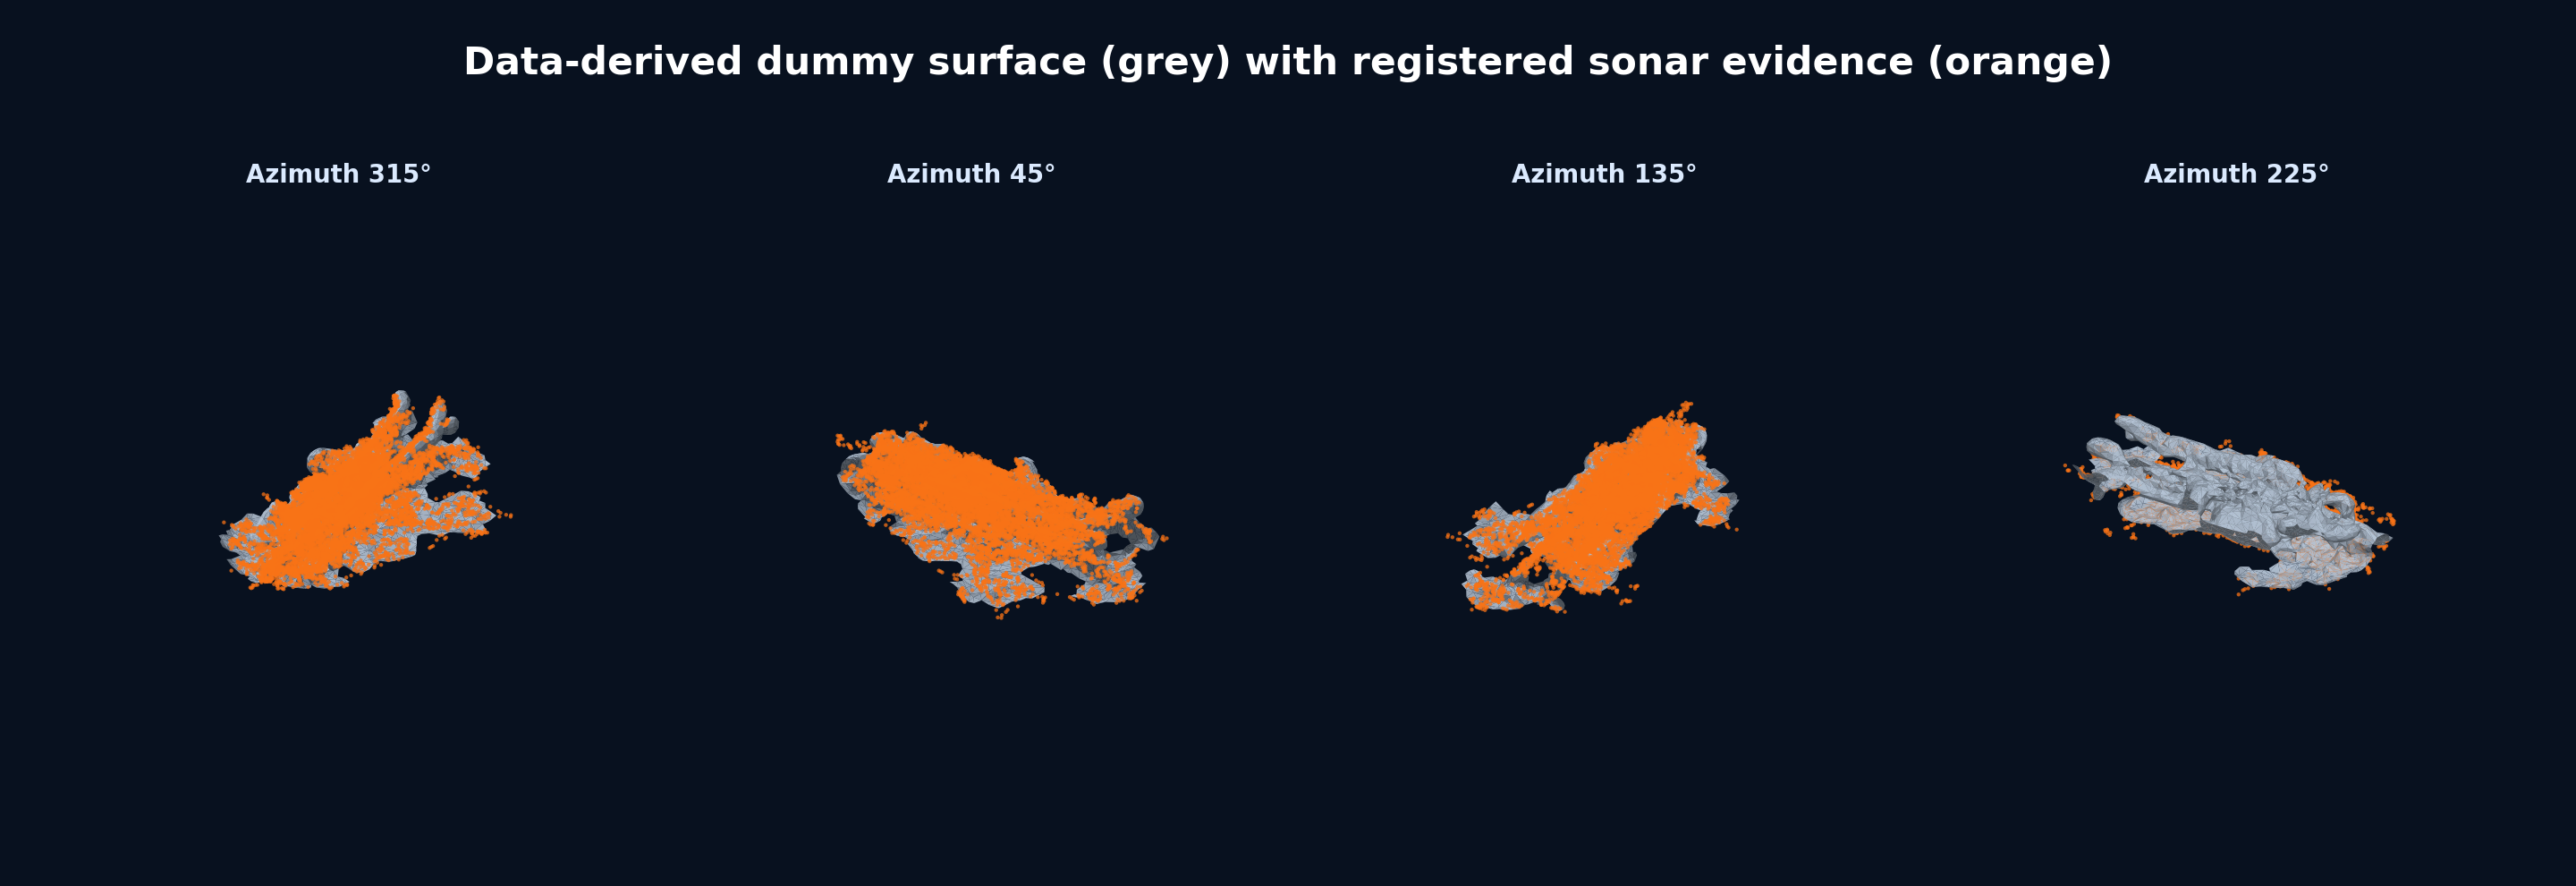
\includegraphics[width=0.98\textwidth]{fig_dummy_turntable.png}
  \caption{Dummy reconstruction turntable. The rear and side views show where
  the measured coverage is thinnest and where Poisson and BPA therefore
  diverge most.}
  \label{fig:dummy_turntable}
\end{figure}

\section{Variant results}
\label{sec:resultsA_variants}

The two variants of \secref{sec:routea_variants} were run on the chair and
tyre, the two categories with the strongest segmentation. Their metrics are
reported in \tabref{tab:routeA_metrics}. The metric
\emph{observed-to-surface} measures, for every accepted registered return, its
distance to the reconstructed surface; a small median means the surface is
faithful to the measurements. \emph{Surface supported} is the fraction of
surface points with a measured return within a support radius (40~mm for the
view-aware variant, the support limit for the TSDF).

\begin{table}[H]
  \centering
  \small
  \begin{adjustbox}{max width=\textwidth}
  \begin{tabular}{@{}lcccccc@{}}
    \toprule
    Variant & Object & Accepted cases & Fused returns & Median (mm) & P95 (mm) & Supported \\
    \midrule
    View-aware SE(2) & Chair & 7 & 972 & 4.14 & 19.31 & 0.63 ($\le 20$~mm) \\
    View-aware SE(2) & Tyre  & 3 & 5{,}000 & 2.91 & 15.82 & 1.00 ($\le 40$~mm) \\
    Ray TSDF & Chair & 2 & 2{,}205 & 2.92 & 9.89 & 1.00 \\
    Ray TSDF & Tyre  & 5 & 7{,}982 & 4.99 & 20.05 & 1.00 \\
    \bottomrule
  \end{tabular}
  \end{adjustbox}
  \caption{Surface-fit metrics for the two \routeA{} variants. Median
  observed-to-surface residuals of $2.9$--$5.0$~mm confirm that the fused
  surfaces sit tightly on the registered returns; the P95 values show that a
  small tail of returns (often multipath or mis-segmented points) lies a few
  centimetres off. ``Supported'' is the fraction of surface within the stated
  radius of a measured return.}
  \label{tab:routeA_metrics}
\end{table}

\begin{itemize}
  \item \textbf{View-aware SE(2).} The chair accepted 7 of its candidate
  cases (972 fused returns) with a median residual of 4.14~mm; the tyre
  accepted 3 (5{,}000 returns) with median 2.91~mm and essentially total
  surface support within 40~mm. The small accepted-case counts are the honest
  cost of the explicit acceptance gate: cases whose planar fit is weak are
  rejected rather than silently fused.
  \item \textbf{Ray TSDF.} The sonar-native variant fused 2,205 chair returns
  from 2 views and 7,982 tyre returns from 5 views into 4--5~mm voxel grids.
  Its surfaces are the most conservative: unsupported vertices are removed, so
  the fraction of multiview-supported surface is only 0.176 (chair) and 0.499
  (tyre) --- the TSDF reports \emph{per-vertex} how many views support it,
  which is exactly the coverage information a sonar reconstruction should
  provide.
\end{itemize}

\subsection{Model-assisted hybrid outputs}
For completeness, the project also produced ``recognizable'' hybrid outputs in
which a dimensionally constrained template (folding chair, parametric tyre)
completes the registered evidence. These are \emph{model-assisted}, not
measurement-derived: the chair completion places inferred frame members
between measured joints, and the tyre completion uses the measured width with a
parametric profile. The tyre hybrid's larger residuals (median 18.5~mm,
P95 65.8~mm) quantify the cost of forcing a template onto sparse evidence, and
make clear why the purely measured variants are preferred for claims of
geometric accuracy.

\section{Interpretation: what these numbers do and do not prove}
\label{sec:resultsA_interpretation}

The numbers above establish four things rigorously:

\begin{enumerate}
  \item \textbf{Pipeline completion.} All five categories completed the full
  registration$\to$fusion$\to$meshing chain; the graphs are fully connected
  (24/24 views), so no object was abandoned.
  \item \textbf{Measurement consistency.} Median observed-to-surface residuals
  of a few millimetres mean that, wherever the sonar did measure, the fused
  surface agrees with the measurements at a scale comparable to the
  segmentation and registration tolerances.
  \item \textbf{Multi-view benefit.} The large loop-closure counts and the
  visual agreement across turntable views show that the fused model is
  self-consistent, which a single scan cannot be.
  \item \textbf{Uncertainty localisation.} The systematic Poisson-vs-BPA
  divergence in the least-supported regions (chair underside, tyre inner wall,
  dummy rear) is a map of where the reconstruction is extrapolated rather than
  measured.
\end{enumerate}

What the numbers do \emph{not} prove is absolute geometric accuracy: there is
no external CAD or scanned reference in \suop{}, so ``4~mm residual'' is a
self-consistency figure, not an error against truth. Likewise, mesh vertex
counts are indicators of pipeline behaviour, not quality. These caveats are
central to the discussion in \secref{ch:discussion} and motivate the
calibrated-acquisition future work of \secref{ch:conclusions}.

% =====================================================================
% Chapter 8 — Route B Results
% =====================================================================
\chapter{Route~B Results}
\label{ch:resultsB}

This chapter reports the results of \routeB{}. It presents the training
progress of the three main runs (\secref{sec:resultsB_training}), the
qualitative epoch-by-epoch evidence for the dummy and drum
(\secref{sec:resultsB_epochs}), the inference behaviour on a real \suop{}
chair segment (\secref{sec:resultsB_chair}), and an interpretation of what the
loss curves do and do not prove (\secref{sec:resultsB_interpretation}).

\section{Training progress}
\label{sec:resultsB_training}

\tabref{tab:routeB_training} reports the training and validation Chamfer loss
of the three principal runs. All runs used the RTX~4060 Laptop GPU, batch size
32--48, Adam at learning rate $10^{-3}$ and 6000 training pairs with a 10\%
hold-out.

\begin{table}[H]
  \centering
  \small
  \begin{adjustbox}{max width=\textwidth}
  \begin{tabular}{@{}lccccccc@{}}
    \toprule
    Run & Data & Epochs & CD@ep1 & CD@final & Val CD@ep1 & Val CD@final & Total time \\
    \midrule
    Dummy (mesh-cond.) & \texttt{dataset\_dummy\_suop} & 10 & 0.03993 & 0.00112 & 0.00459 & 0.00073 & 1705~s \\
    Drum & \texttt{dataset\_drum\_suop} & 10 & 0.01435 & 0.00178 & 0.00362 & 0.00051 & 1642~s \\
    Chair & procedural & 150 & 0.01657 & 0.00228 & 0.00159 & 0.00048 & 14{,}827~s \\
    \bottomrule
  \end{tabular}
  \end{adjustbox}
  \caption{Route~B training summary. Symmetric Chamfer loss $L =
  \mathrm{CD}(C,G)+\mathrm{CD}(F,G)$ on unit-normalised clouds. All three runs
  converge: the final training CD is 1--2 orders of magnitude below its
  epoch-1 value, and validation CD stays below training CD, indicating no
  memorisation at the sampled checkpoints.}
  \label{tab:routeB_training}
\end{table}

The dummy run (trained on \routeA{}-mesh-conditioned pairs) shows the fastest
relative improvement, dropping from 0.03993 to 0.00112 within ten epochs; the
drum converges from a lower starting point (0.01435) to 0.00178. The chair
run, trained for 150 epochs, reaches a training CD of $2.28\times10^{-3}$
while the validation CD plateaus around $5\times10^{-4}$ after epoch 45 ---
the typical signature of a model that has learned the coarse structure and is
only polishing fine detail.

\section{Epoch-by-epoch evidence}
\label{sec:resultsB_epochs}

The epoch contact sheets (\figref{fig:dummy_epochs}, \figref{fig:drum_epochs})
render, for every epoch, the same three panels: the sonar-like partial input,
the complete reference (ground truth) and the network's fine completion.
Reading a sheet left-to-right shows the input, the truth, and what the network
produces from the input alone --- a direct visual check that the completion is
actually derived from the partial rather than from a memorised shape.

\begin{figure}[H]
  \centering
  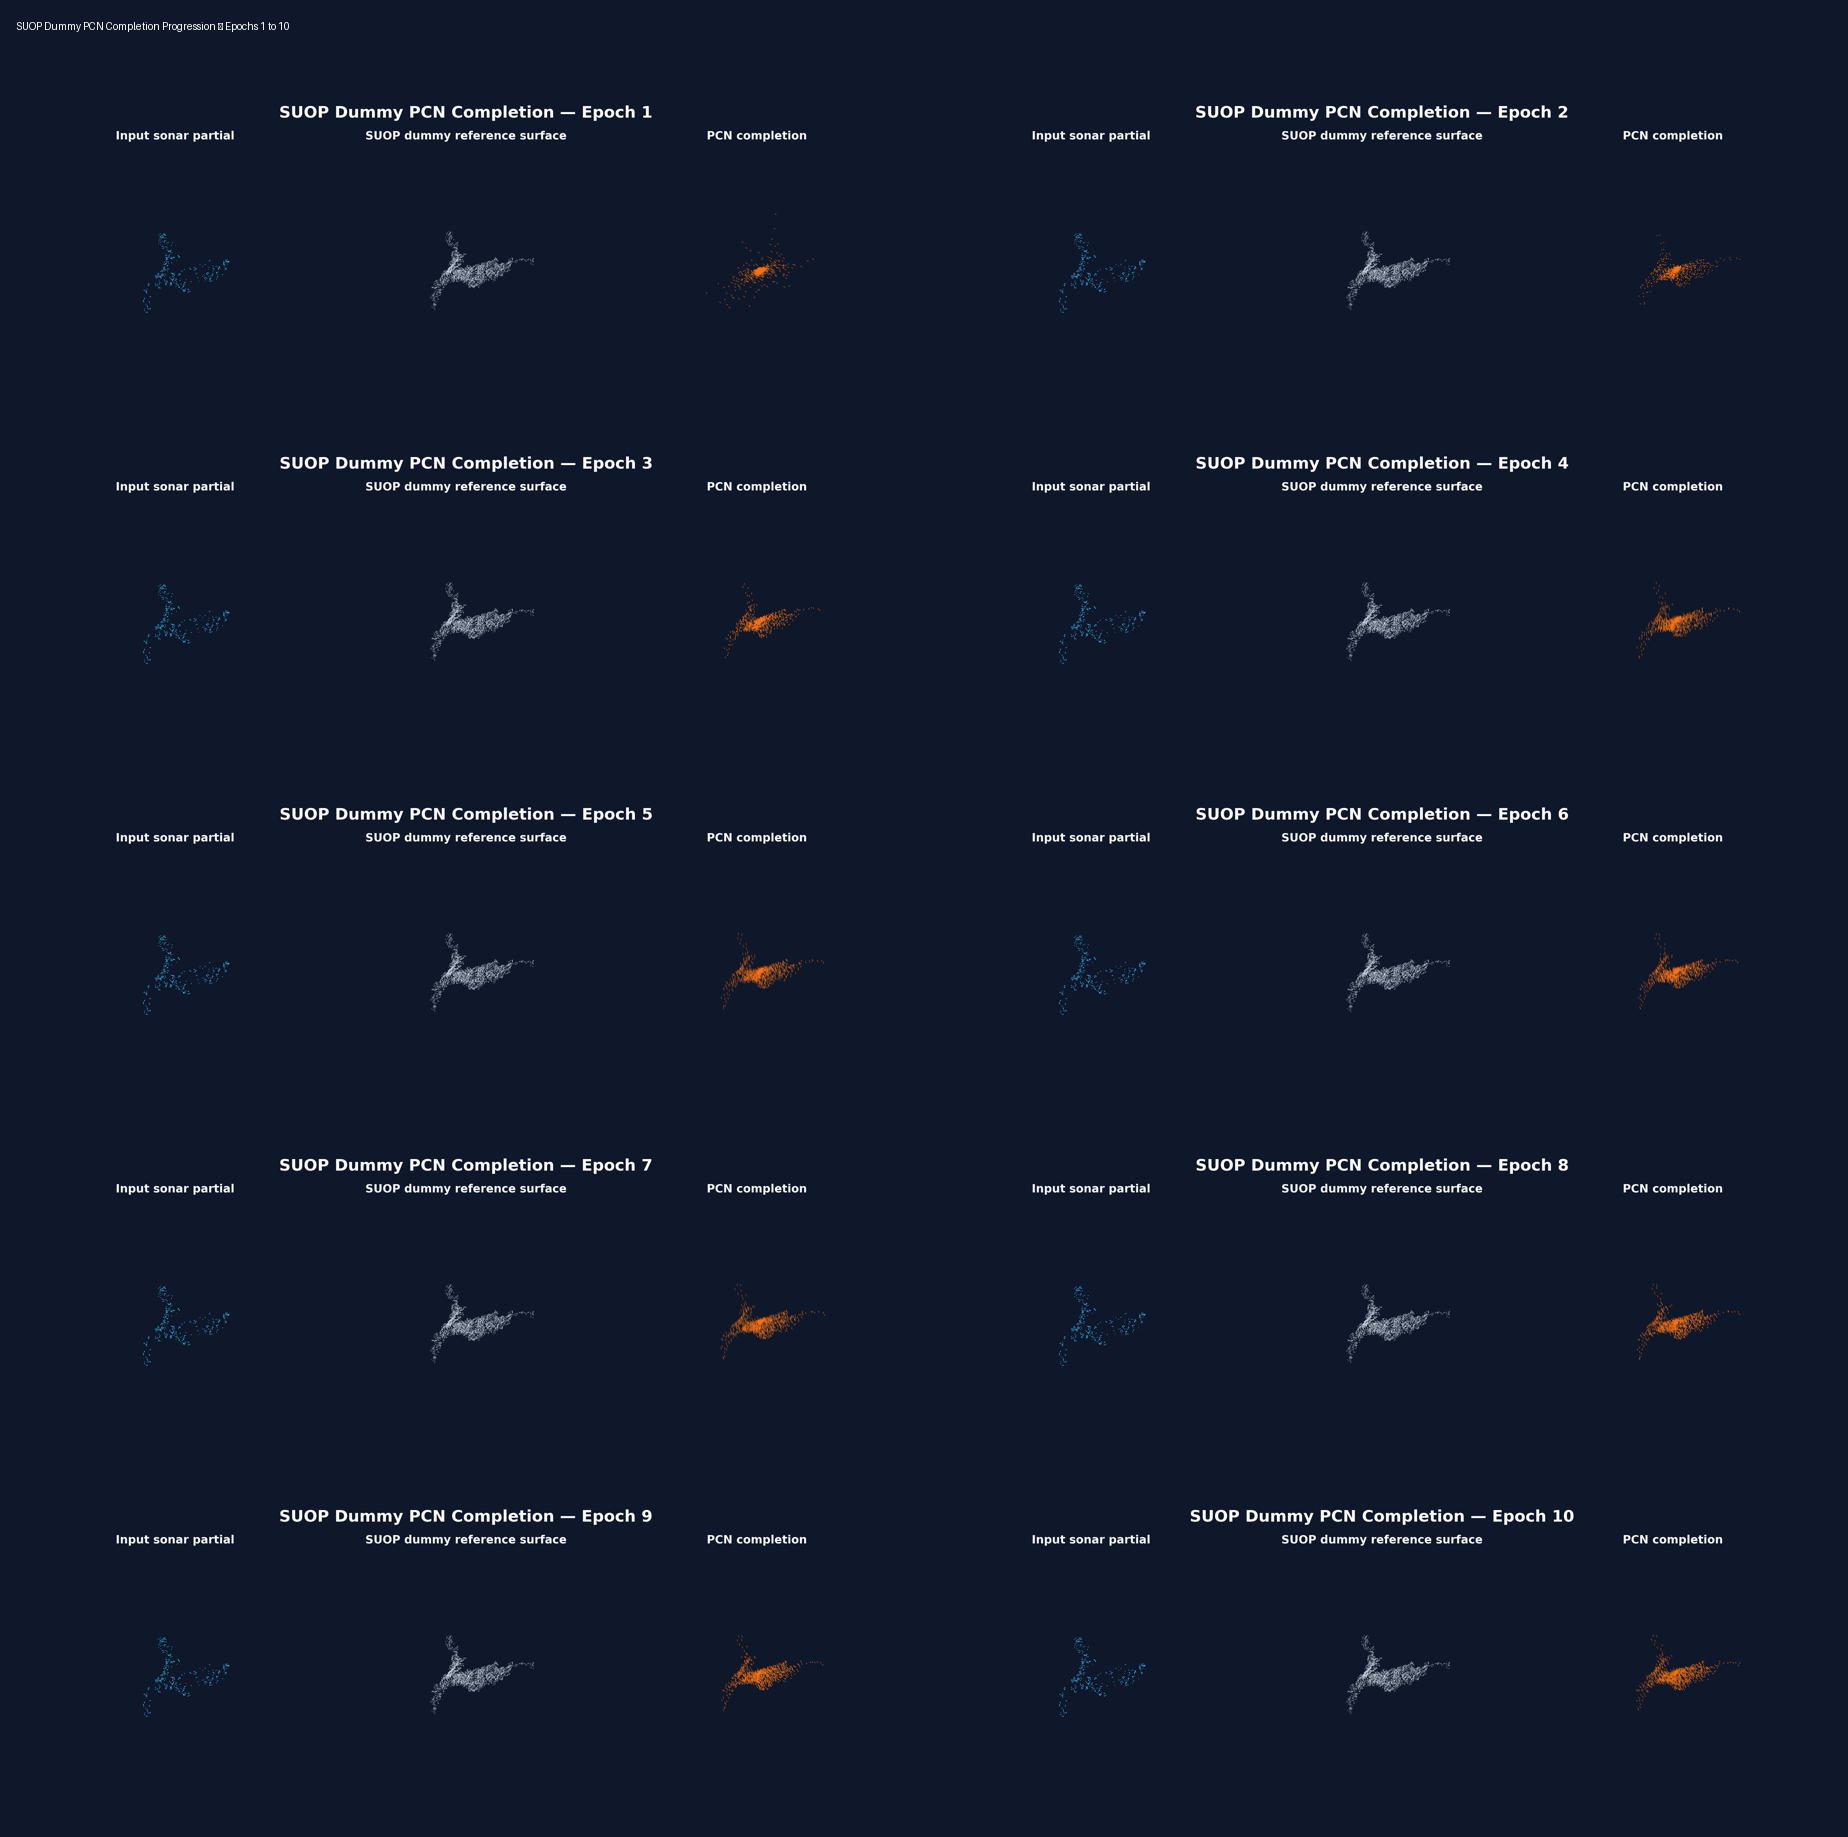
\includegraphics[width=0.88\textwidth]{fig_dummy_epochs.png}
  \caption{Dummy \routeB{} training progression, epochs 1--10 (mesh-conditioned
  run). Each row shows the same semantic triple: partial input, complete
  reference, network completion. The completion evolves from a rough blob
  (epoch 1) to a recognisable mannequin silhouette with limbs (epoch 10).}
  \label{fig:dummy_epochs}
\end{figure}

\begin{figure}[H]
  \centering
  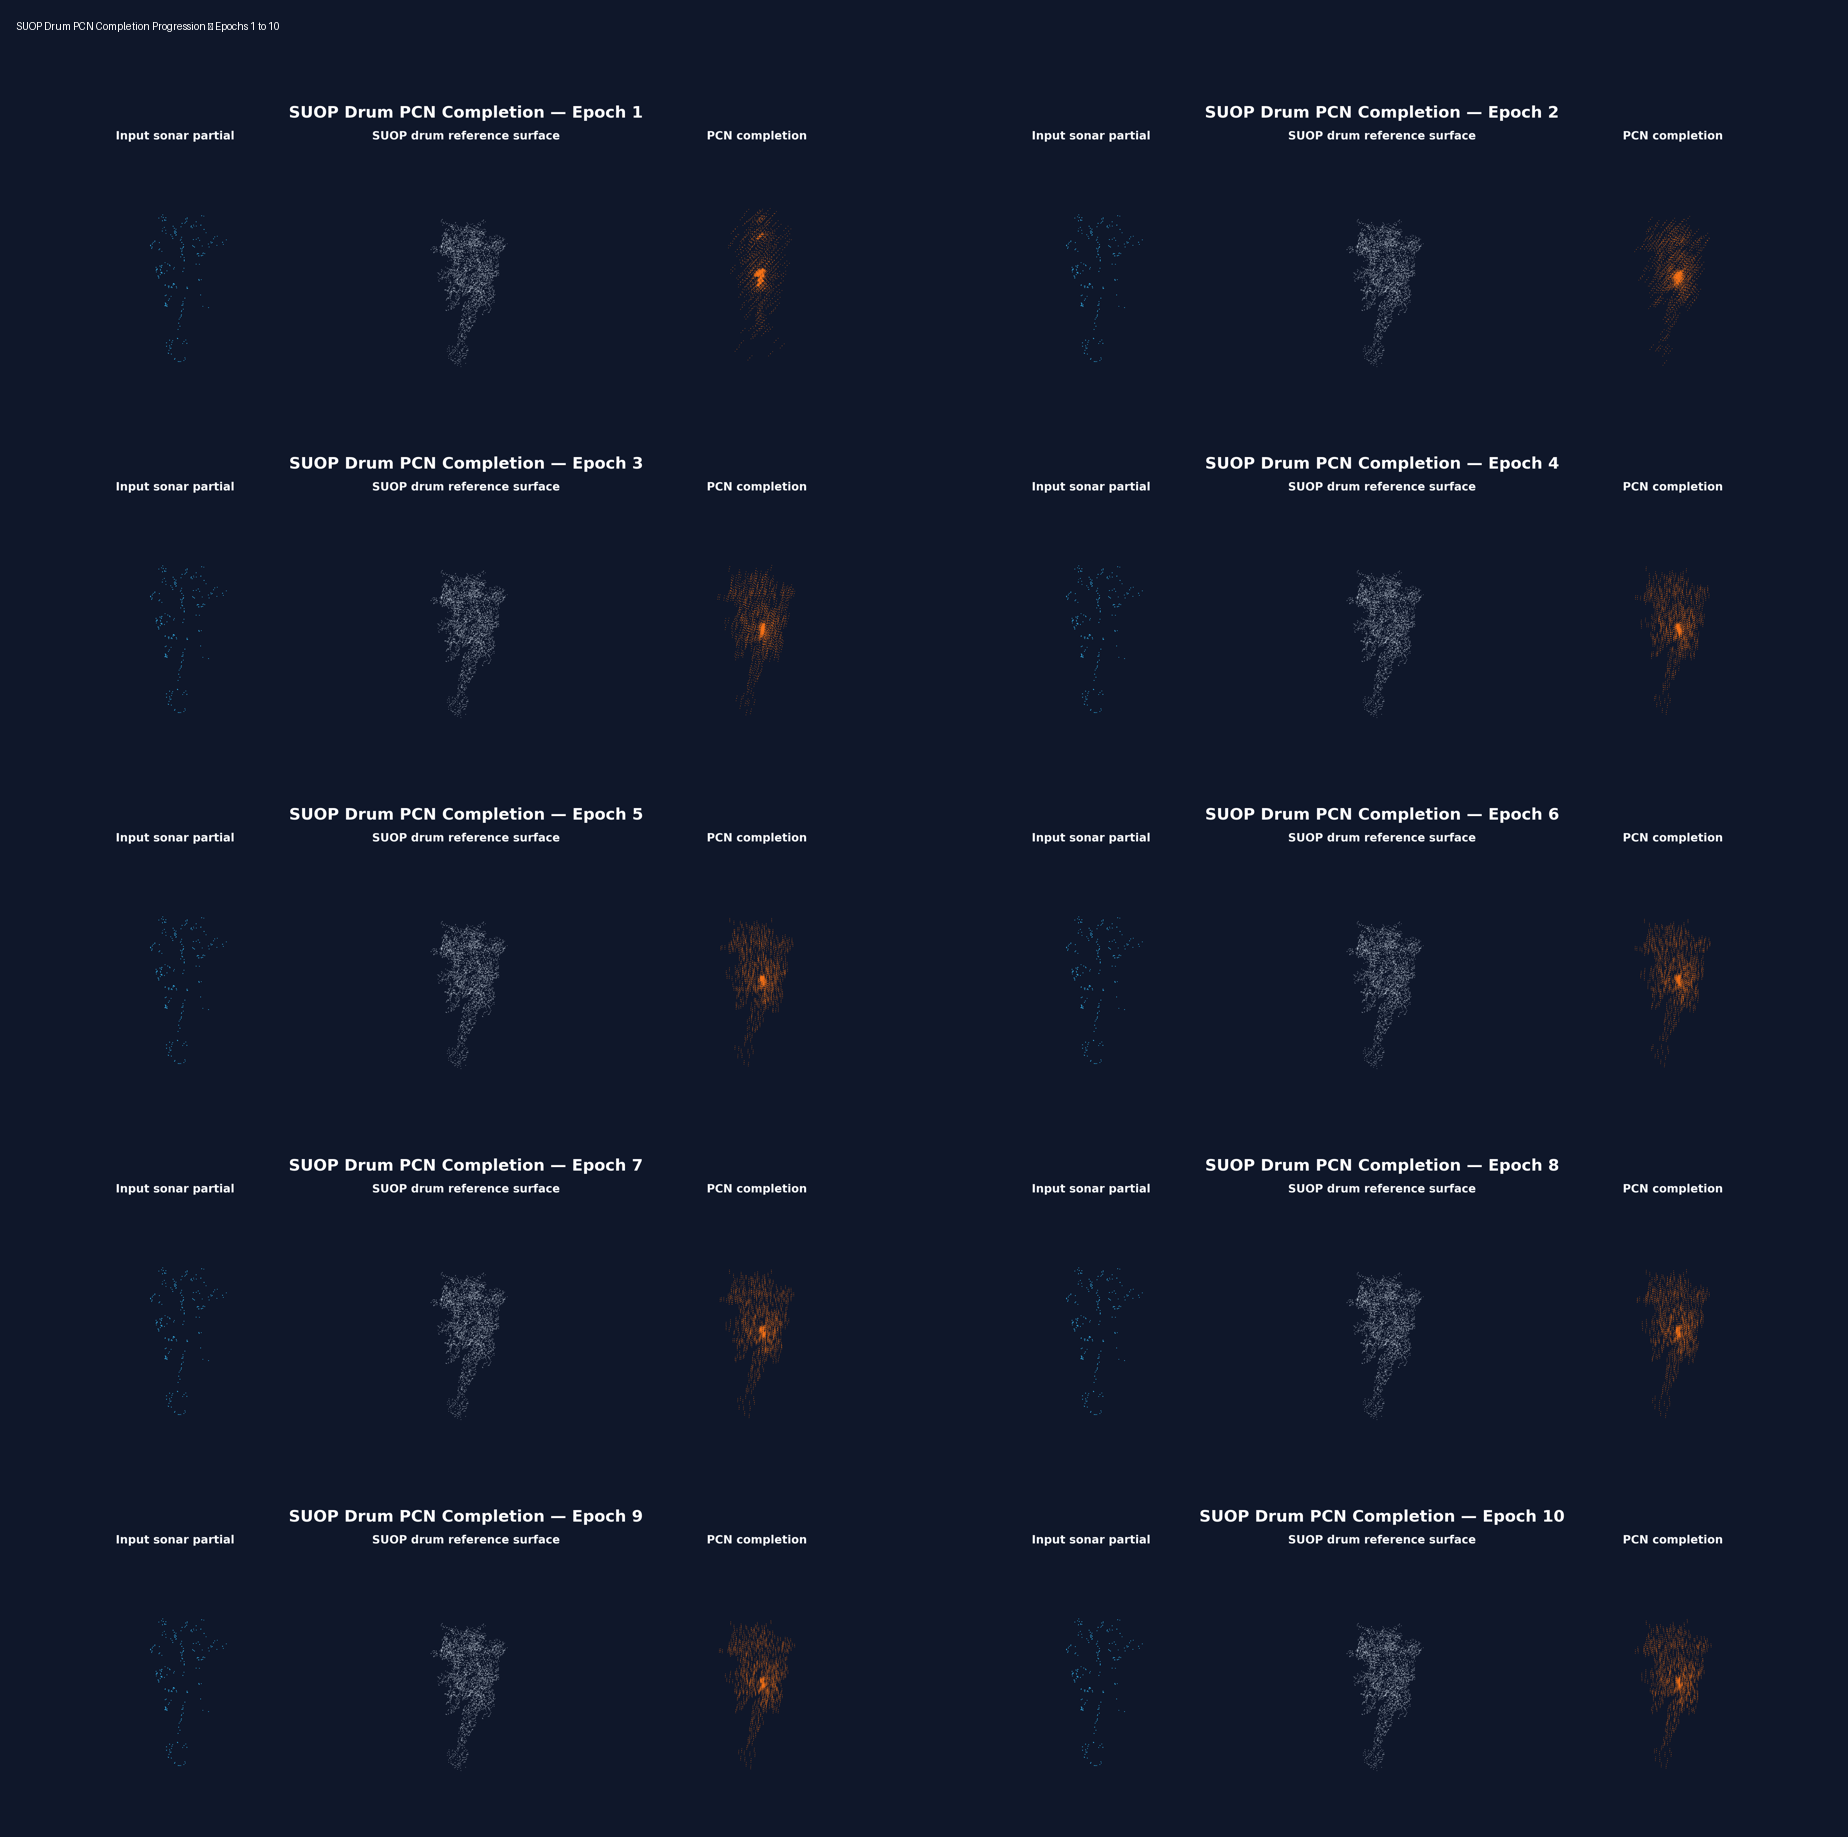
\includegraphics[width=0.88\textwidth]{fig_drum_epochs.png}
  \caption{Drum \routeB{} training progression, epochs 1--10. The cylindrical
  barrel and end caps emerge early; later epochs refine the end-cap rims and
  reduce blur at the edges of the completion.}
  \label{fig:drum_epochs}
\end{figure}

\figref{fig:dummy_ep05_vs_10} compares epoch 5 and epoch 10 for the dummy
directly: the mid-training completion has the correct gross proportions but
softer limbs, while the epoch-10 completion is crisper and closer to the
reference silhouette.

\begin{figure}[H]
  \centering
  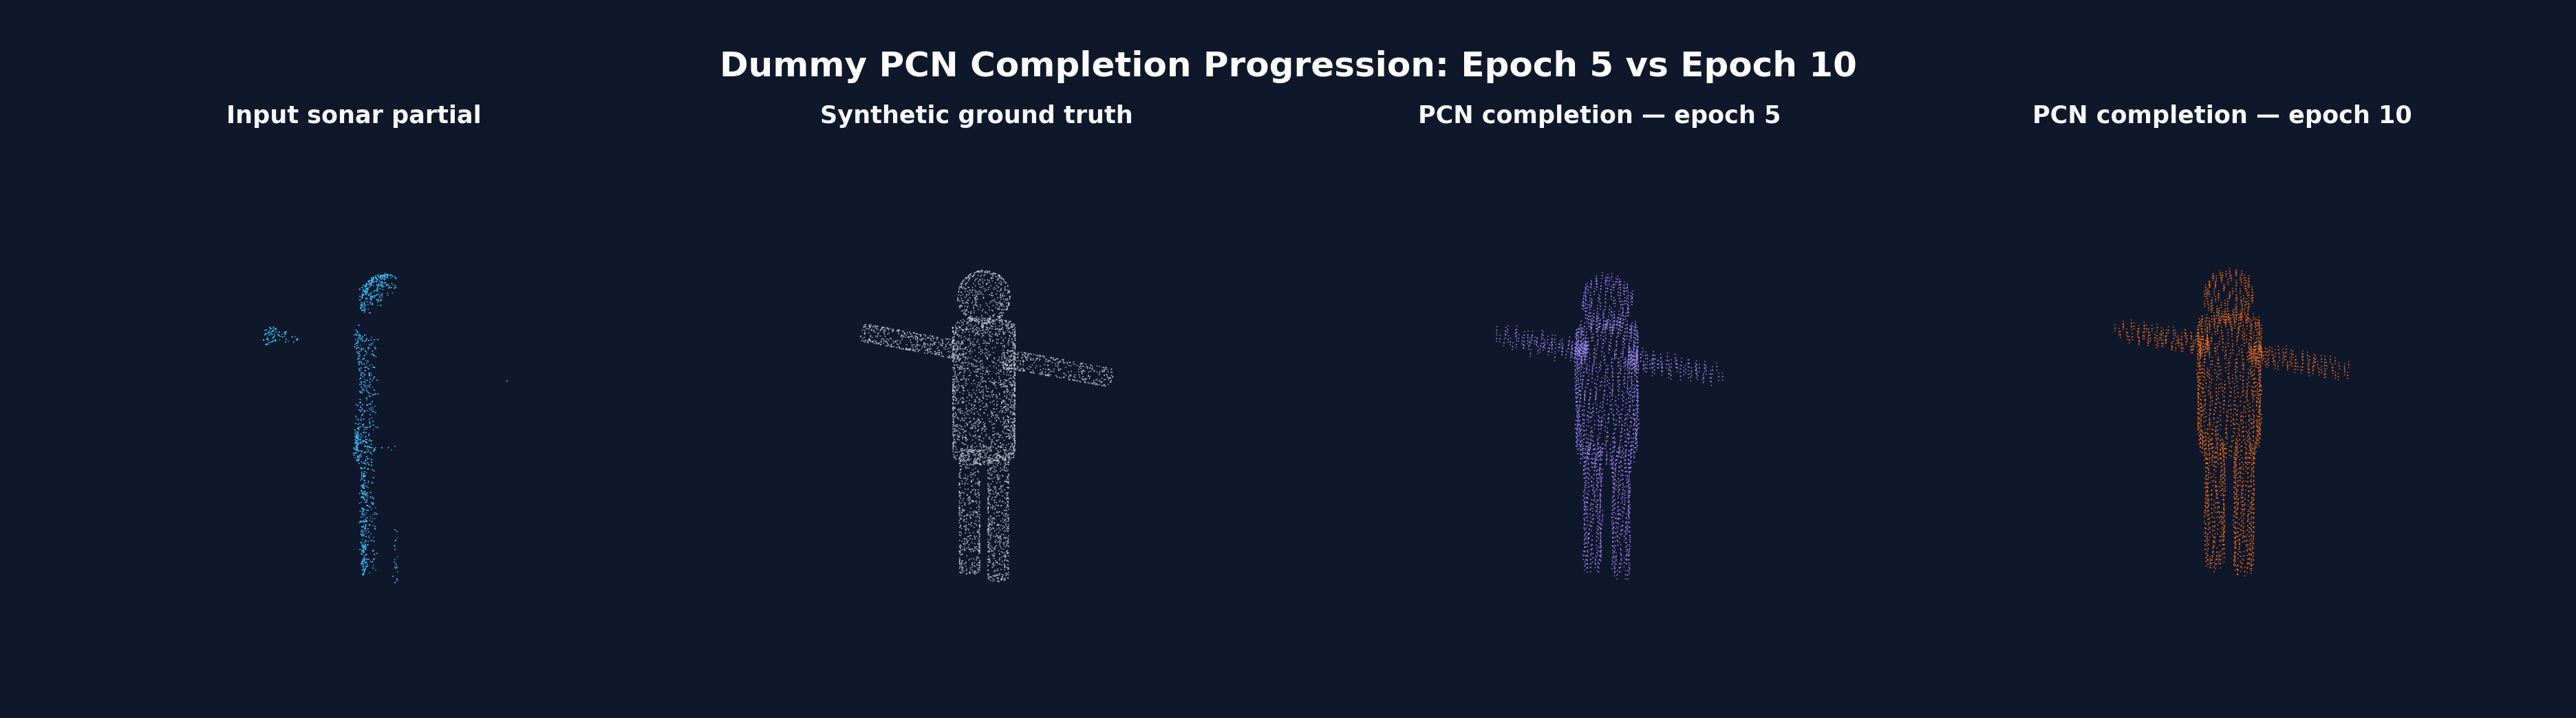
\includegraphics[width=0.98\textwidth]{fig_dummy_ep05_vs_10.png}
  \caption{Dummy completion at epoch 5 versus epoch 10 (top to bottom: input,
  reference, completion; left column epoch 5, right column epoch 10). The
  later checkpoint sharpens the shoulder/arm junctions and legs.}
  \label{fig:dummy_ep05_vs_10}
\end{figure}

\section{Inference on a real SUOP partial}
\label{sec:resultsB_chair}

The trained chair checkpoint (\texttt{pcn\_chair.pth}) was applied to a real
\suop{} chair segment --- a single unprocessed partial view, the deployment
scenario that \routeB{} was designed for. \figref{fig:chair_pcn_progression}
shows the input and the completions at epochs 1 and 15.

\begin{figure}[H]
  \centering
  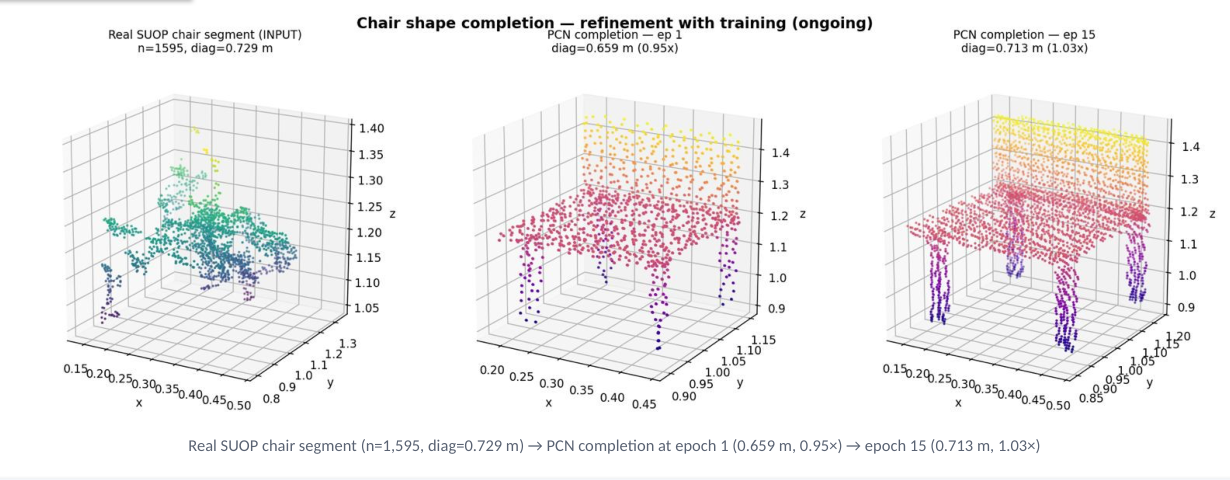
\includegraphics[width=0.98\textwidth]{fig_chair_pcn_progression.png}
  \caption{Route~B chair inference on a real \suop{} partial: input segment
  (1{,}595 points, 0.729~m diagonal), PCN completion at epoch 1 (0.659~m
  diagonal) and at epoch 15 (0.713~m diagonal). The completion grows toward the
  input scale while adding inferred structure in the unobserved regions.}
  \label{fig:chair_pcn_progression}
\end{figure}

Two quantitative observations are worth recording:

\begin{enumerate}
  \item \textbf{Scale recovery.} The completed cloud's bounding-box diagonal
  moves from 0.659~m at epoch 1 to 0.713~m at epoch 15, converging toward the
  0.729~m input diagonal. Because training normalises to the unit sphere, the
  network must \emph{re-learn} the absolute scale of the object category; the
  convergence of the output diagonal toward the input diagonal is evidence
  that it does.
  \item \textbf{Completeness.} The completion emits a full 4096-point (fine)
  cloud from a 1{,}595-point partial, filling the far side, the underside and
  parts of the frame that the single view never measured. This is the defining
  behaviour of \routeB{} and the direct contrast with \routeA{}'s open,
  evidence-limited output.
\end{enumerate}

\section{Interpretation: what these numbers do and do not prove}
\label{sec:resultsB_interpretation}

The results establish the following:

\begin{enumerate}
  \item \textbf{The architecture trains.} All runs reduce Chamfer loss
  substantially and monotonically, and validation stays below training,
  showing the PCN with coarse-to-fine decoding and folding is trainable on
  this data.
  \item \textbf{The prior is category-shaped.} The epoch sheets show the
  completions take on the correct category anatomy (mannequin silhouette,
  barrel shape, chair frame), which only a learned prior can supply from a
  partial view.
  \item \textbf{Inference generalises to real sonar.} The real chair partial
  is completed at the correct scale, and the result is visually coherent.
\end{enumerate}

What the numbers do \emph{not} prove is physical accuracy of the inferred
geometry. The Chamfer loss is computed against \emph{synthetic} references, so
a low loss means ``consistent with the training distribution'', not
``correct against the real object''. A visually plausible completion can be a
hallucination --- the network may interpolate between training shapes rather
than recover the actual object. The dummy's mesh-conditioned training set
mitigates this by matching the sensor's geometry distribution, but the real
\suop{} objects have no external scan with which to verify the completions.
This threat to validity is addressed in \secref{ch:discussion} and the future
work of \secref{ch:conclusions}.

% =====================================================================
% Chapter 9 — Discussion
% =====================================================================
\chapter{Discussion}
\label{ch:discussion}

This chapter interprets the results of both routes, discusses the coverage of
evidence across the five object categories (\secref{sec:disc_coverage}), the
threats to validity (\secref{sec:disc_threats}), and the implications of the
project's central claim --- that the two routes answer different questions and
must be judged accordingly (\secref{sec:disc_implications}).

\section{What the results mean together}
\label{sec:disc_together}

Taken together, the results of \secref{ch:resultsA} and \secref{ch:resultsB}
support the dissertation's thesis: the two routes are complementary answers
that succeed precisely where the other route's assumption fails.

\routeA{} demonstrates that \emph{when overlapping views exist}, sonar
partials can be aligned into a self-consistent measured model: 24/24 views per
object were connected by pose-graph optimisation, median measured-to-surface
residuals of $2.9$--$5.0\mm$ were achieved by the variants, and the
Poisson/BPA pair provides an honest map of where the evidence is thin. The
price is completeness: unobserved regions are empty or explicitly trimmed, and
the model is only as good as the registration.

\routeB{} demonstrates that \emph{when only one view exists}, a learned prior
can still produce a complete object representation: the PCN converged on all
runs (final training CD $1.1\times10^{-3}$--$2.3\times10^{-3}$), the epoch
sheets show category-shaped completions, and a real chair partial was
completed at the correct scale. The price is fidelity: the inferred geometry is
a hypothesis from the training distribution, not a measurement.

The interesting result is the \emph{mesh-conditioned dummy}: training \routeB{}
on \routeA{} meshes transferred the measured geometry into the learned prior.
This is the strongest evidence that the routes are partners rather than rivals
--- the geometric route's best output becomes the learned route's training
ground, closing a loop between measurement and inference.

\section{Coverage across categories}
\label{sec:disc_coverage}

Evidence is not uniform across the five categories, and the dissertation is
explicit about that (\tabref{tab:coverage}).

\begin{table}[H]
  \centering
  \small
  \begin{adjustbox}{max width=\textwidth}
  \begin{tabular}{@{}p{1.6cm}p{6.3cm}p{6.3cm}@{}}
    \toprule
    Object & \routeA{} (geometric fusion) & \routeB{} (PCN completion) \\
    \midrule
    Chair & Rich: segments, fused cloud, Poisson + BPA, turntable, view-aware
    and ray-TSDF variants, hybrid & Checkpoint (150~ep) + real-partial
    inference shown \\
    Tyre & Rich: segments, reconstruction, turntable, view-aware and ray-TSDF
    variants, hybrid & No dedicated PCN result in this workspace \\
    Dummy & Good: segments, mesh comparison, turntable & Rich: mesh-conditioned
    training, epochs 1--10, comparisons \\
    Drum & Numerically complete: fused cloud and meshes; no dedicated render &
    Rich: epochs 1--10, contact sheet, comparisons \\
    Net & Numerically complete: fused cloud and meshes; no dedicated render &
    No checkpoint or completion image \\
    \bottomrule
  \end{tabular}
  \end{adjustbox}
  \caption{Result coverage across categories. The pipelines completed
  numerically for all five objects; rendered evidence is richest for
  chair/tyre/dummy. The table is a transparency statement, not a quality
  ranking.}
  \label{tab:coverage}
\end{table}

Two points follow. First, \emph{numerical completion} (files produced, graphs
connected, losses decreased) and \emph{validated quality} (independent
reference, external ground truth) are different things; this dissertation has
much more of the former than the latter, as \suop{} allows. Second, the
category coverage asymmetry is a consequence of where the segmentation is
reliable: the chair and tyre produce compact, scale-consistent clusters,
whereas the net's mesh-like structure and the drum's large planar barrel make
segmentation harder or the renders less informative. Future work should fill
the drum/net evidence gaps deliberately.

\section{Threats to validity}
\label{sec:disc_threats}

\subsection{Internal validity}
The main internal threats concern the correctness of the pipelines themselves:

\begin{enumerate}
  \item \textbf{Registration correctness.} FPFH can confuse repeated parts
  (chair legs, tyre tread), and RANSAC can accept a symmetric but wrong
  alignment. The pipeline mitigates this with the fitness $\geq 0.25$ edge
  gate, MST initialisation, loop closures and edge pruning, but it cannot
  prove correctness without ground-truth poses. The graph-connectivity and
  fitness statistics show \emph{consistency}, not \emph{correctness}.
  \item \textbf{Segmentation leakage.} If the object segment contains seabed
  or rig points, registration fits them too. The elevation gating and
  scale-consistent clustering in \secref{ch:dataset} reduce this, but residual
  contamination is likely for the sparse 10~m cases (which were excluded from
  fusion precisely for this reason).
  \item \textbf{Evaluation metric choice.} Chamfer distance rewards uniform
  coverage and can hide local error; counting mesh vertices rewards pipeline
  completion, not quality. Both metrics are used here with their limitations
  stated explicitly rather than presented as accuracy.
\end{enumerate}

\subsection{External validity}
The largest external threat is that \suop{} provides \emph{no external
ground truth} for geometry: no CAD models, no logged object poses, and no
independent scan of the physical objects. Consequences:

\begin{enumerate}
  \item \routeA{}'s ``residual'' figures are self-consistency measures. A
  surface could sit perfectly on noisy returns and still be wrong about the
  real object (e.g.\ a consistently biased sound speed shifts all ranges).
  \item \routeB{}'s training references are synthetic (procedural or
  \routeA{}-derived). The learned prior is therefore a prior over
  \emph{our models of the objects}, not over the real objects. Completeness of
  the inference cannot be validated on the real data.
  \item The object was moved by hand between \suop{} cases; any motion blur or
  non-rigid deformation during acquisition becomes a bias that neither route
  can model.
\end{enumerate}

\subsection{Reliability and reproducibility}
All experiments used pinned open-source versions (Open3D 0.19, PyTorch, NumPy,
scikit-learn; see Appendix~\ref{app:environment}) and were run from
reproducible batch scripts with logged output. The datasets
(\texttt{dataset\_*.npz}) are deterministic given the seed, and the
registration and meshing manifests are committed as JSON in the project, so
every table in this dissertation can be reproduced from the scripts and
inputs. The main reliability caveat is compute: the pairwise registration cost
($\sim$15--18 minutes per object) and the 150-epoch chair run ($\sim$4.1~h)
limit how many configurations could be explored.

\section{Implications for practice}
\label{sec:disc_implications}

Three practical recommendations follow from the results:

\begin{enumerate}
  \item \textbf{Choose the route by data availability, not fashion.} For
  inspection-grade geometry where a measured answer is required, invest in
  multi-view acquisitions and use \routeA{}. For single-pass deployments where
  a complete model is needed, train a category-specific \routeB{} model.
  \item \textbf{Report uncertainty honestly.} The Poisson/BPA divergence map
  (\routeA{}) and the training-distribution caveat (\routeB{}) should travel
  with the results; an unqualified mesh or completion overstates certainty.
  \item \textbf{Link the routes.} The mesh-conditioned training result shows
  that the geometric route's outputs can bootstrap the learned route's prior.
  This hybridisation is a more productive research direction than treating the
  two routes as competitors.
\end{enumerate}

\section{Summary}
\label{sec:disc_summary}

The results are consistent with the dissertation's central claim: \routeA{}
produces measured, self-consistent but partial geometry when views exist;
\routeB{} produces complete, prior-informed but unverified geometry when only
one view exists; and the two can be chained. The principal limitation --- the
absence of external geometric ground truth in \suop{} --- motivates the
concluding chapter's proposed experiment.

% =====================================================================
% Chapter 10 — Conclusions and Future Work
% =====================================================================
\chapter{Conclusions and Future Work}
\label{ch:conclusions}

This chapter concludes the dissertation. It restates what was built and what
was learned (\secref{sec:conc_summary}), maps the results back to the research
question and objectives (\secref{sec:conc_objectives}), and proposes the
experiments that would convert this project's self-consistency evidence into
externally validated accuracy (\secref{sec:conc_future}).

\section{Summary of contributions}
\label{sec:conc_summary}

This dissertation set out to answer how incomplete acoustic-sonar returns of
small underwater objects, as provided by the \suop{} dataset, can be converted
into useful 3D representations --- and to make the choice between two
reconstruction paradigms explicit. The project delivered:

\begin{enumerate}
  \item \textbf{An honest data audit.} The \suop{} release was characterised
  as a detection dataset: a fixed BlueView BV5000, an object moved by hand,
  no logged poses, truncated ping exports. Every design decision in the
  project follows from these facts (\secref{ch:dataset}).
  \item \textbf{A complete preparation pipeline.} Extraction, denoising,
  plane removal, temporal background rejection and scale-consistent clustering
  converted 120 raw cases into clean per-object segments, with a curated
  24-view subset per object for fusion (\secref{ch:dataset}).
  \item \textbf{\routeA{} --- multi-view geometric fusion.} A fully geometric
  pipeline (FPFH/RANSAC/ICP $\to$ pose graph with MST and loop closures $\to$
  fusion $\to$ Screened Poisson + BPA) ran successfully on all five
  categories: 24/24 views connected per object, fused clouds of 7--100\,k
  points, and two clean meshes per object. Two hardened variants --- a
  seabed-plane-constrained SE(2) registration and a sonar-native first-return
  ray TSDF with explicit per-vertex measurement support --- achieved median
  observed-to-surface residuals of $2.9$--$5.0\mm$ (\secref{ch:resultsA}).
  \item \textbf{\routeB{} --- single-view learned completion.} A PCN with a
  PointNet-style encoder and a coarse-to-fine folding decoder was trained with
  a symmetric Chamfer loss on sonar-realistic partials. The training data came
  from procedural models \emph{and} from \routeA{}'s own meshes, linking the
  routes. All runs converged (final training CD $1.1\times10^{-3}$--
  $2.3\times10^{-3}$), epoch sheets show category-shaped completions, and a
  real chair partial was completed at the correct scale
  (\secref{ch:resultsB}).
  \item \textbf{An explicit route rationale.} The conditions under which each
  route is the right answer, and the difference in what their outputs mean,
  were stated precisely and compared side by side (\secref{ch:comparison}).
\end{enumerate}

\section{Answers to the research question and objectives}
\label{sec:conc_objectives}

Returning to the research question of \secref{sec:research_question}:

\begin{quote}
\emph{How can incomplete acoustic-sonar returns of small underwater objects,
as provided by the \suop{} dataset, be converted into a useful 3D object
representation, and which reconstruction route should be chosen under which
data-availability conditions?}
\end{quote}

The answer, supported by the results, is twofold.

\emph{How to convert the returns:} by treating segmentation as a first-class
problem (the object must be separated from a dominant seabed), estimating
object poses from geometry rather than reading them from an encoder, and then
choosing between fusion and completion. When multiple views exist, FPFH/RANSAC/
ICP plus pose-graph optimisation reliably aligns the partials into a
self-consistent measured model. When only one view exists, a PCN trained on
sonar-realistic (partial, complete) pairs --- grounded where possible in the
geometric route's meshes --- produces a complete, category-shaped point cloud.

\emph{Which route to choose:} \routeA{} whenever overlapping views of a rigid
object are available and the output must be a faithful record of measurements
(inspection, safety assessment); \routeB{} whenever only one view exists and a
complete representation is required (classification features, simulation
targets, manipulation). The routes are complementary; their outputs differ in
completeness, in the status of unobserved regions, and in the availability of
ground truth; and they must therefore be evaluated with different protocols.

Against the six objectives of \secref{sec:research_question}: O1 (data
characterisation) is met in \secref{ch:dataset}; O2 (preparation pipeline) in
\secref{ch:dataset}; O3 (\routeA{}) in \secref{ch:routeA} and
\secref{ch:resultsA}; O4 (\routeB{}) in \secref{ch:routeB} and
\secref{ch:resultsB}; O5 (route rationale) in \secref{ch:comparison}; and O6
(evaluation and future work) across \secref{ch:resultsA}--\secref{ch:discussion}
and the remainder of this chapter.

\section{Limitations}
\label{sec:conc_limitations}

The limitations already detailed in \secref{ch:discussion} are summarised here
as the boundary of what can be claimed:

\begin{enumerate}
  \item \textbf{No external geometric ground truth.} \suop{} provides no CAD
  models, no logged object poses and no independent scan. All \routeA{}
  accuracy claims are therefore self-consistency measures, and \routeB{}
  completions cannot be verified against the real objects.
  \item \textbf{Uneven evidence.} The drum and net categories completed the
  pipelines numerically but lack dedicated rendered validation, and only
  chair/tyre received the view-aware and ray-TSDF variant treatment.
  \item \textbf{Compute-bounded exploration.} The pairwise registration cost
  and the multi-hour chair run limited the number of configurations
  (thresholds, voxels, network sizes) that could be swept.
\end{enumerate}

\section{Future work}
\label{sec:conc_future}

\subsection{A calibrated multi-view acquisition with external reference}
The single most valuable next step is to re-acquire the five \suop{} object
categories under a \emph{pose-calibrated} protocol, as proposed in the
project's acquisition specification (\texttt{SUOP\_ACQUISITION\_RECONSTRUCTION.md}):

\begin{enumerate}
  \item Keep the object rigid and fixed; move the sonar, or place the object
  on a non-reflective indexed turntable.
  \item Log the full calibrated $SE(3)$ transform for every scan (encoder or
  survey accuracy $\approx 2$~mm and $0.2^\circ$ at the 3~m working range).
  \item Acquire 24 azimuths at $15^\circ$ spacing at the 3~m range, in two
  elevation bands (the \suop{} $45^\circ$ close-range setup and a
  $15$--$25^\circ$ grazing setup), so that chair legs, seat undersides and
  tyre sidewalls are observed.
  \item Record background-only scans before and after the sequence, full
  per-ping pan/tilt/time/sound-speed metadata, and sound-speed profiles at
  start and end.
  \item Scan the same objects with a high-resolution optical or laser system
  (or use the manufacturer's CAD) to obtain an \emph{external} reference mesh.
\end{enumerate}

With logged poses, the pose-estimation stage of \routeA{} is bypassed and the
raw first-return rays can be integrated directly into a 3--5~mm TSDF, giving a
\emph{measured} reference. With the external scan, both routes can be
evaluated quantitatively on the same objects:

\begin{itemize}
  \item \routeA{}: Chamfer distance and F-score between the fused/TSDF surface
  and the external mesh; registration error against the logged poses; coverage
  as the fraction of the external surface within a tolerance.
  \item \routeB{}: Chamfer distance and F-score of the completions against the
  external mesh on \emph{held-out real partials} --- this is the definitive
  test of whether the learned prior generalises to genuine sonar rather than
  simulated partials.
\end{itemize}

\subsection{Hardening each route}
Independent of the new acquisition, each route can be hardened:

\begin{itemize}
  \item \routeA{}: integrate the later-return (multipath) evidence through
  cross-view consistency instead of discarding it at source; add an explicit
  outlier-rejection pass in the TSDF; and expose per-vertex coverage as a
  standard output (already prototyped in the ray-TSDF variant).
  \item \routeB{}: evaluate against held-out \emph{real} partials with
  F-score; replace the fixed 4096-point fine output with a
  density-adaptive decoder (e.g.\ FoldingNet-style
  \citep{yang2018folding} or a transformer-based completion
  \citep{xie2020pointr}); and train a multi-category model that reports
  category uncertainty.
\end{itemize}

\subsection{Chaining the routes}
Finally, the mesh-conditioned training result suggests a promising hybrid:
use \routeA{} to build a library of measured meshes per category, use those
meshes (not procedural models) to train \routeB{}, and use \routeB{}'s
completions as \emph{priors} inside a revised \routeA{} (e.g.\ as soft
regularisers in the TSDF). This would give the geometric route the
completeness it lacks and the learned route the sensor-grounded prior it
needs --- the most productive direction this dissertation can point towards.

\section{Closing remark}
\label{sec:conc_closing}

Underwater sonar is a hard sensor: its point clouds are partial, noisy and
unevenly sampled, and the \suop{} dataset adds the further difficulty of
unlogged object pose. This dissertation shows that two complementary routes
can nevertheless convert such returns into useful 3D representations --- one
that faithfully fuses what was measured when several views exist, and one that
inferentially completes what was not observed when only a single view exists.
The two routes are not competitors; they are the two halves of a complete
answer, and the next acquisition campaign with logged poses and external
reference will let both halves be measured against the truth they ultimately
serve.


% ------------------------- references -------------------------------
\clearpage
\bibliographystyle{IEEEtran}
\bibliography{references}

% ------------------------- appendices -------------------------------
\clearpage
\appendix
\input{chapters/appendix_a}
\input{chapters/appendix_b}

\end{document}
